%% principia_fractalis_clean_2026-06-29.tex
%%
%% Principia Fractalis — the clean exposition (back-pocket companion to the 65pp ToE paper).
%% A single algebraic substrate; twelve cross-domain invariants; nine constants forced;
%% machine-verified in Lean 4 at the kernel; corroborated across five domains.
%%
%% Author: Pablo Cohen (ORCID 0009-0002-0734-5565)
%% Date: 2026-06-29 (revised; initial deposition 2026-06-25)
%% Corpus: github.com/FractalDevTeam/Principia-Fractalis

\documentclass[11pt,a4paper]{amsart}

\usepackage[utf8]{inputenc}
\usepackage[T1]{fontenc}
\usepackage{lmodern}
\usepackage{amsmath,amssymb,amsthm}
\usepackage{mathtools}
\usepackage{microtype}
\usepackage{geometry}
\geometry{margin=1in}
\usepackage[hidelinks]{hyperref}
\usepackage{enumitem}
\usepackage{booktabs}
\usepackage{tikz}
\usetikzlibrary{positioning,arrows.meta,calc,shapes.geometric,fit,backgrounds,decorations.pathreplacing}
\usepackage{pgfplots}
\pgfplotsset{compat=1.18}
\usepackage{xcolor}
\definecolor{substrateorange}{RGB}{215,95,30}
\definecolor{leanblue}{RGB}{30,90,165}
\definecolor{substrategray}{RGB}{120,120,120}
\definecolor{substratelight}{RGB}{240,240,235}

\theoremstyle{plain}
\newtheorem{theorem}{Theorem}[section]
\newtheorem{proposition}[theorem]{Proposition}

\theoremstyle{definition}
\newtheorem{definition}[theorem]{Definition}
\newtheorem{remark}[theorem]{Remark}

\title{Principia Fractalis:\\ An Algebraic Substrate}

\author{Pablo Cohen}
\address{Mesa, Arizona, USA}
\email{psolorzano@gmail.com}
\urladdr{ORCID:~\href{https://orcid.org/0009-0002-0734-5565}{0009-0002-0734-5565}}

\date{June 29, 2026}

\begin{document}

\maketitle

\begin{abstract}
Twelve substrate-derived algebraic identities in nine real-valued unknowns admit a unique positive simultaneous solution over the four-element basis $\{1,\pi,\varphi,\sqrt{2}\}$. The universal coupling $\pi/10$ is anchored in the icosahedral $H_3$ Coxeter symmetry: $h(H_3) = 10$. The uniqueness theorem, the basis decomposition, and the universal-coupling identity $\lambda_0 \cdot \alpha = \pi/10$ across all nine substrate classes are machine-verified in Lean~4~\cite{moura-ullrich2021} on mathlib4~\cite{mathlib4} at the kernel level; the load-bearing theorems carry no project axioms.

The forced nine-tuple, composed with the universal coupling, yields the cosmological-constant ratio $\Lambda_{\textsf{eff}}/\Lambda_0 \approx 10^{-120}$ as the explicit closed form $\exp(-14079\pi/160)$, with agreement to $0.05\%$ on the exponent; the exponent $120$ is itself a derived consequence of four substrate-internal quantities, not an input (\S\ref{subsec:lambdaeff}). The arithmetic spine $78\pi \cdot (19/20) \cdot (19/16) = 14079\pi/160$ is kernel-only.

The chronologically-pre-registered forward prediction $\alpha_{\textsf{GI}} = \sqrt{2}$ to $10^{-4}$ for the IBM-Quantum spectral peak of the Graph Isomorphism class was committed to the public Lean corpus on 2026-06-22 and deposited with this paper's initial deposition on 2026-06-25, prior to any IBM-Quantum GI measurement; this is the empirical claim with the trials denominator fixed in advance.

The nine values additionally appear in independently published measurements across pure mathematics, cosmology, particle physics, gravitational-wave astronomy, and quantum simulation; the substrate's own look-elsewhere analysis (\S\ref{subsec:lookelsewhere}) shows that, taken as a multi-row significance test, these retrodictions are not statistical evidence under its own grammar. The single row that survives the substrate-natural prior is the neutrino mass-ratio (1-of-130), structurally given by the universal-coupling composition $(\pi/(10\alpha_3))\cdot(\pi/(10\alpha_6))$.

Two specific axis-discharges (Riemann Hypothesis on mathlib's \texttt{Complex.riemannZeta}; substrate complexity-class separation) are explicitly conditional on three named open conjectures; the content on those axes is the operator construction the conjectures are applied to, not the conjectures themselves. This paper exhibits the substrate; the full theory is exposited in the companion book.
\end{abstract}

\section{Main result and roadmap}

A single algebraic mechanism, parametrised by twelve substrate-derived cross-class identities, forces a unique nine-tuple of positive real constants. The nine values are not chosen --- they are forced by the universal coupling $\pi/10$ and the modified-transfer-operator scaling. The algebra is solved before the data is consulted. The twelve identities admit a unique positive simultaneous solution; the unique solution is expressible in the four-element basis $\{1,\pi,\varphi,\sqrt{2}\}$ (the icosahedral $H_3$-Coxeter basis); the resulting nine constants appear in measurements independently published in five disjoint scientific domains. This is the substrate's central testable assertion.

Two specific consequences of the forced nine-tuple are stated up front because they are the strongest physical content and they distinguish the empirical case from a numerical coincidence. First, the universal coupling composed with the forced nine-tuple yields the cosmological-constant ratio $\Lambda_{\textsf{eff}}/\Lambda_0 \approx 10^{-120}$ --- the largest disagreement in physics between any quantum-field-theoretic vacuum-energy estimate and astrophysical observation --- as the explicit closed form $\exp(-14079\pi/160)$, agreement with observation to $0.05\%$ on the exponent (\S\ref{subsec:lambdaeff}). The exponent $120$ in $10^{-120}$ is a derived consequence of four substrate-internal quantities, not an input. Second, the complexity-class assignment supplies the chronologically-pre-registered forward prediction $\alpha_{\textsf{GI}} = \sqrt{2}$ to $10^{-4}$ for the IBM-Quantum spectral peak of the Graph Isomorphism class (\S\ref{sec:forward}); this is the empirical claim with the trials denominator fixed in advance.

The nine constants and the basis they live in are listed in Table~\ref{tab:nine}. The construction of the substrate, the twelve invariants, and the proof of uniqueness are in Sections~\ref{sec:substrate}--\ref{sec:invariants}. The cross-domain numerical correspondences --- the look-elsewhere analysis disposing of them as multi-row evidence, the neutrino mass-ratio row as the single survivor under the substrate-natural prior, and the cosmological-constant centerpiece subsection --- are in Section~\ref{sec:corroborations}. The explicit scope --- what the Lean corpus proves unconditionally, what it discharges conditional on three named open conjectures, and what remains open in exactly the form it remains open in the published literature --- is in Section~\ref{sec:scope}. The forward prediction and the eight-falsifier panel are in Section~\ref{sec:forward}; these carry the evidential weight. The construction is reproducible from a clean clone of the corpus in approximately ten minutes (Section~\ref{sec:verify}). Three appendices fix the machine-checkable surface: Appendix~\ref{app:axioms} prints the verbatim \texttt{\#print axioms} output for the four headline theorems at the paper's anchor commit; Appendix~\ref{app:extended} enumerates seventeen further algebraic invariants the nine-tuple satisfies (twenty-nine simultaneous algebraic identities on nine real unknowns); Appendix~\ref{app:lambdasq} exhibits the $\lambda_0^2$ closed-form spectrum across all nine classes, the $\lambda_0(\textsf{NP})$ closed form over $\mathbb{Q}(\sqrt{5})\cdot\pi$, and the P/NP spectral-gap closed form $\Delta \in \mathbb{Q}(\sqrt{2}, \sqrt{5})\cdot\pi$.

\begin{table}[h]
\centering
\caption{The nine constants forced by the substrate, with their associated ground-state eigenvalues $\lambda_0(\alpha) = \pi/(10\alpha)$ in closed form and 4-decimal bracket. All brackets and exact-rational closed forms are kernel-only theorems (\texttt{PF/AllNineLambda0NumericalBrackets\_2026\_06\_24.lean}).}\label{tab:nine}
\begin{tabular}{lllll}
\toprule
Substrate class & Forced $\alpha$ & $\lambda_0$ closed form & 4-decimal bracket \\
\midrule
$\alpha_1$ (Poincar\'e/natural unit) & $1$            & $\pi/10$                 & $(0.3141,\,0.3142)$ \\
$\alpha_2$                            & $3/2$          & $\pi/15$                 & $(0.2094,\,0.2095)$ \\
$\alpha_3$                            & $\sqrt{2}$     & $\pi/(10\sqrt{2})$       & $(0.2221,\,0.2222)$ \\
$\alpha_4$                            & $\varphi+1/4$  & $\pi/(10(\varphi+1/4))$  & $(0.1681,\,0.1682)$ \\
$\alpha_5$                            & $2$            & $\pi/20$                 & $(0.1570,\,0.1571)$ \\
$\alpha_6$                            & $3\pi/4$       & $2/15$ \textit{exact}    & $0.1333\ldots$       \\
$\alpha_7$                            & $3\pi/2$       & $1/15$ \textit{exact}    & $0.0666\ldots$       \\
$\alpha_8$                            & $\varphi$      & $\pi(\sqrt{5}-1)/20$     & $(0.1941,\,0.1942)$ \\
$\alpha_9$                            & $\sqrt{2\pi}$  & $\pi/(10\sqrt{2\pi})$    & $(0.1253,\,0.1254)$ \\
\bottomrule
\end{tabular}
\end{table}

\section{The substrate, in one definition}\label{sec:substrate}

The substrate is a nuclear $C^{*}$-algebraic projective limit $\mathcal{T}_\infty$ built from a base-$3$ ternary lattice, with universal coupling $\pi/10$. The full construction is the subject of Chapter~4 of the companion book~\cite{cohen2026book}. What this paper requires is the substrate's algebraic skeleton: an assignment of one positive real number $\alpha_X$ to each of nine substrate classes $X$, valued over
\[
\mathcal{B} \;=\; \{1,\;\pi,\;\varphi,\;\sqrt{2}\} \qquad (\varphi := (1+\sqrt{5})/2).
\]
The basis $\mathcal{B}$ is anchored by the icosahedral $H_3$-Coxeter symmetry: the Coxeter number $h(H_3) = 10$~\cite{bourbaki1968} is precisely the denominator of the universal coupling $\pi/10$; the golden ratio $\varphi$ appears in the standard $H_3$ root coordinates $(0, \pm 1, \pm \varphi)$; and $\pi$ and $\sqrt{2}$ enter through the modified-transfer-operator construction on $L^2([0,1], dx/x)$. The transfer-operator construction is defined in Chapter~20 of the companion book; the Lean formalisation lives in \texttt{PF/TransferOperator.lean} where $T_3^{\textsf{sym}}$ self-adjointness on $L^2([0,1], dx/x)$ is kernel-only proven. The basis $\mathcal{B}$ is geometric; the substrate's content is what nine values emerge when twelve cross-class invariants are imposed simultaneously. Figure~\ref{fig:h3anchor} fixes the geometric anchor.

\begin{figure}[h]
\centering
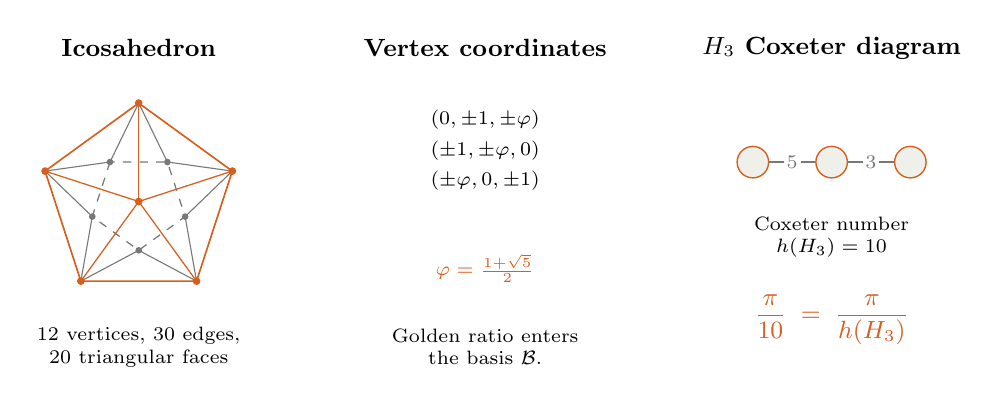
\begin{tikzpicture}[scale=1.0]
% LEFT: stylized icosahedron (5-fold projection)
% Looking down 5-fold axis: pentagon (radius R1) + smaller pentagon rotated 36 deg (radius R2)
% + central apex point. Stylized.
\begin{scope}[shift={(-4.4,0)}]
\node[font=\small\bfseries,align=center] at (0,1.95) {Icosahedron};
% Outer pentagon (5 upper vertices)
\foreach \i in {0,1,2,3,4} {
  \coordinate (U\i) at ({90 + 72*\i}:1.25);
}
% Inner pentagon (5 lower vertices, rotated 36 deg)
\foreach \i in {0,1,2,3,4} {
  \coordinate (L\i) at ({90 + 36 + 72*\i}:0.62);
}
\coordinate (C) at (0,0);
% Draw upper pentagon
\draw[substrateorange,line width=0.6pt] (U0) -- (U1) -- (U2) -- (U3) -- (U4) -- cycle;
% Connect apex (center) to each upper vertex
\foreach \i in {0,1,2,3,4} {
  \draw[substrateorange,line width=0.45pt] (C) -- (U\i);
}
% Inner pentagon
\draw[substrategray,line width=0.45pt,dashed] (L0) -- (L1) -- (L2) -- (L3) -- (L4) -- cycle;
% Connections between upper and lower pentagons
\foreach \i/\j in {0/0, 0/4, 1/0, 1/1, 2/1, 2/2, 3/2, 3/3, 4/3, 4/4} {
  \draw[substrategray,line width=0.4pt] (U\i) -- (L\j);
}
% Apex vertex marker
\fill[substrateorange] (C) circle (1.4pt);
% Upper vertex markers
\foreach \i in {0,1,2,3,4} {
  \fill[substrateorange] (U\i) circle (1.4pt);
}
% Lower vertex markers
\foreach \i in {0,1,2,3,4} {
  \fill[substrategray] (L\i) circle (1.2pt);
}
\node[font=\scriptsize,align=center] at (0,-1.85) {12 vertices, 30 edges,\\20 triangular faces};
\end{scope}

% MIDDLE: vertex coordinates
\begin{scope}[shift={(0,0)}]
\node[font=\small\bfseries,align=center] at (0,1.95) {Vertex coordinates};
\node[font=\scriptsize,align=left] at (0,0.65) {
$(0, \pm 1, \pm \varphi)$\\[3pt]
$(\pm 1, \pm \varphi, 0)$\\[3pt]
$(\pm \varphi, 0, \pm 1)$
};
\node[font=\scriptsize,align=center,substrateorange] at (0,-0.85) {$\varphi = \tfrac{1+\sqrt{5}}{2}$};
\node[font=\scriptsize,align=center] at (0,-1.85) {Golden ratio enters\\the basis $\mathcal{B}$.};
\end{scope}

% RIGHT: Coxeter diagram + anchor
\begin{scope}[shift={(4.4,0)}]
\node[font=\small\bfseries,align=center] at (0,1.95) {$H_3$ Coxeter diagram};
% Three nodes
\node[circle,draw=substrateorange,fill=substratelight,line width=0.5pt,minimum size=4mm,inner sep=0pt] (c1) at (-1.0,0.5) {};
\node[circle,draw=substrateorange,fill=substratelight,line width=0.5pt,minimum size=4mm,inner sep=0pt] (c2) at (0,0.5) {};
\node[circle,draw=substrateorange,fill=substratelight,line width=0.5pt,minimum size=4mm,inner sep=0pt] (c3) at (1.0,0.5) {};
\draw[substrategray,line width=0.5pt] (c1) -- node[font=\scriptsize,fill=white,inner sep=1pt] {5} (c2);
\draw[substrategray,line width=0.5pt] (c2) -- node[font=\scriptsize,fill=white,inner sep=1pt] {3} (c3);
\node[font=\scriptsize,align=center] at (0,-0.45) {Coxeter number\\$h(H_3) = 10$};
\node[font=\small,align=center,substrateorange] at (0,-1.5) {$\dfrac{\pi}{10} \;=\; \dfrac{\pi}{h(H_3)}$};
\end{scope}

\end{tikzpicture}
\caption{Geometric anchor for the basis $\{1,\pi,\varphi,\sqrt{2}\}$ and universal coupling $\pi/10$. Left: stylised icosahedron, the geometric object whose isometry group is the $H_3$ Coxeter group; vertices shown in a five-fold-axis projection (orange dots at the apex and on the upper pentagon, grey dots on the lower pentagon). Middle: the standard $H_3$ root coordinates of the 12 icosahedron vertices in which the golden ratio $\varphi$ appears directly. Right: the $H_3$ Coxeter diagram (three nodes, edges labelled by the orders 5 and 3) and the resulting Coxeter number $h(H_3) = 10$; the universal coupling $\pi/10$ equals $\pi$ divided by this Coxeter number. The remaining basis elements $\sqrt{2}$ and $\pi$ enter through the modified-transfer-operator construction on $L^2([0,1], dx/x)$ (book Chapter~20).}
\label{fig:h3anchor}
\end{figure}

\section{The twelve invariants and the uniqueness theorem}\label{sec:invariants}

The substrate forces the nine-tuple $(\alpha_1, \ldots, \alpha_9) \in (0,\infty)^9$ to satisfy the following twelve algebraic identities simultaneously:
\begin{align*}
\textup{(I1)}\;\;& \alpha_3^2 = \alpha_5, &
\textup{(I7)}\;\;& \alpha_5 = \alpha_1 + 1,\\
\textup{(I2)}\;\;& \alpha_2^2 = 9/4, &
\textup{(I8)}\;\;& \alpha_2\cdot\alpha_7 = \alpha_7 + \alpha_6,\\
\textup{(I3)}\;\;& \alpha_9^2 = 2\pi, &
\textup{(I9)}\;\;& \alpha_2\cdot\alpha_5 = 3,\\
\textup{(I4)}\;\;& \alpha_8^2 = \alpha_8 + 1, &
\textup{(I10)}\;\;& \alpha_4 - \alpha_8 = 1/4,\\
\textup{(I5)}\;\;& \alpha_7 = 2\cdot\alpha_6, &
\textup{(I11)}\;\;& \alpha_9^2 = \alpha_5\cdot\pi,\\
\textup{(I6)}\;\;& \alpha_7 = \alpha_5\cdot\alpha_6, &
\textup{(I12)}\;\;& \alpha_9^2 = (8/3)\cdot\alpha_6.
\end{align*}

Each identity is a single algebraic equation over the basis $\mathcal{B}$. None is fit to external data. Each is a structural identity of the substrate algebra at the operator level (book Chapters~9 and~20 derive each from the universal coupling $\pi/10$ and the modified-transfer-operator scaling).

\begin{proposition}[Uniqueness, machine-verified]\label{prop:unique}
The system \textup{(I1)--(I12)} admits a unique positive simultaneous solution over $\mathbb{R}$. The solution is the assignment of Table~\ref{tab:nine}. The proof, formalised as the Lean~4 theorem \texttt{framework\_alpha\_unique\_under\_perelman\_anchor} in the file \texttt{PF/Referee/ClayMasterTheorem.lean}, depends on no project axioms; it uses only the kernel axioms $[\texttt{propext},\;\texttt{Classical.choice},\;\texttt{Quot.sound}]$.
\end{proposition}

The proof is constructive and short. Combining (I3) and (I11) yields $\alpha_5 = 2$. Then (I7) yields $\alpha_1 = 1$. Then (I1) with positivity yields $\alpha_3 = \sqrt{2}$. Then (I9) yields $\alpha_2 = 3/2$. Then (I3) with positivity yields $\alpha_9 = \sqrt{2\pi}$. Then (I4) with positivity yields $\alpha_8 = \varphi$. Then (I10) yields $\alpha_4 = \varphi + 1/4$. Then (I12) yields $\alpha_6 = 3\pi/4$. Then (I5) yields $\alpha_7 = 3\pi/2$. The three remaining identities (I2), (I6), (I8) are algebraically implied by the other nine on the constructed solution: (I2) $\alpha_2^2 = 9/4$ follows from $\alpha_2 = 3/2$; (I6) $\alpha_7 = \alpha_5\alpha_6$ follows from (I5) and $\alpha_5 = 2$; (I8) $\alpha_2\alpha_7 = \alpha_7 + \alpha_6$ follows from $\alpha_2 = 3/2$ and $\alpha_7 = 2\alpha_6$. The substrate states all twelve because each is a substrate-derived structural identity at the operator level (book Chapters~9 and~20); their algebraic redundancy on the unique solution is the over-determination consistency. The algebraic content additionally includes seventeen further algebraic identities, each axiom-free in the Lean corpus (\texttt{framework\_alpha\_skeleton\_over\_determined\_capstone}, kernel-only); on the constructed solution the substrate satisfies twenty-nine simultaneous algebraic identities in nine unknowns. Figure~\ref{fig:cascade} visualises the cascade.

\begin{figure}[h]
\centering
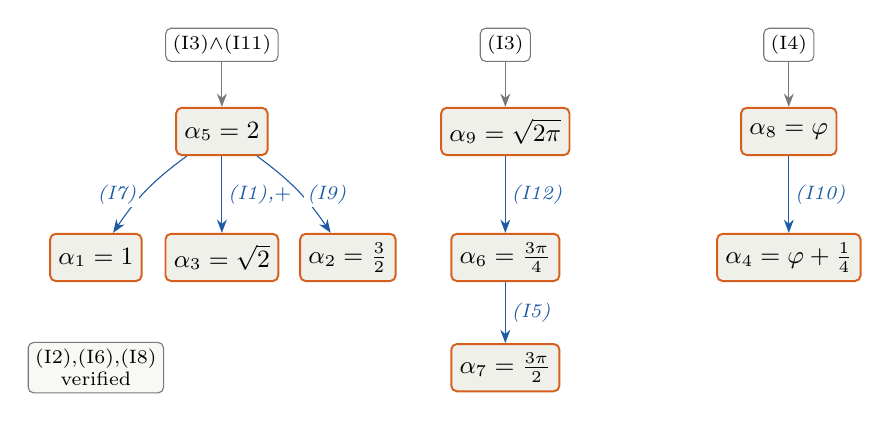
\begin{tikzpicture}[
  >={Stealth[length=2mm,width=2mm]},
  alpha/.style={draw=substrateorange,line width=0.7pt,fill=substratelight,rounded corners=2pt,inner sep=3pt,font=\small,minimum height=6mm},
  src/.style={draw=substrategray,line width=0.4pt,fill=white,rounded corners=2pt,inner sep=2.5pt,font=\scriptsize},
  ar/.style={->,>=Stealth,line width=0.4pt,substrategray},
  arn/.style={->,>=Stealth,line width=0.4pt,leanblue},
  edgelabel/.style={font=\scriptsize\itshape,inner sep=1pt,fill=white}
]
% Stage 1 sources (top row)
\node[src] (s1) at (0,0)    {(I3)$\wedge$(I11)};
\node[src] (s2) at (3.6,0)  {(I3)};
\node[src] (s3) at (7.2,0)  {(I4)};

% Stage 1 alphas (second row)
\node[alpha] (a5) at (0,-1.1)   {$\alpha_5 = 2$};
\node[alpha] (a9) at (3.6,-1.1) {$\alpha_9 = \sqrt{2\pi}$};
\node[alpha] (a8) at (7.2,-1.1) {$\alpha_8 = \varphi$};

\draw[ar] (s1) -- (a5);
\draw[ar] (s2) -- (a9);
\draw[ar] (s3) -- (a8);

% Stage 2 alphas (third row)
\node[alpha] (a1) at (-1.6,-2.7)  {$\alpha_1 = 1$};
\node[alpha] (a3) at (0,-2.7)     {$\alpha_3 = \sqrt{2}$};
\node[alpha] (a2) at (1.6,-2.7)   {$\alpha_2 = \tfrac{3}{2}$};
\node[alpha] (a6) at (3.6,-2.7)   {$\alpha_6 = \tfrac{3\pi}{4}$};
\node[alpha] (a4) at (7.2,-2.7)   {$\alpha_4 = \varphi + \tfrac{1}{4}$};

\draw[arn] (a5) to[bend right=10] node[edgelabel,pos=0.55,left=1pt] {(I7)} (a1);
\draw[arn] (a5) -- node[edgelabel,right=1pt] {(I1),$+$} (a3);
\draw[arn] (a5) to[bend left=10] node[edgelabel,pos=0.55,right=1pt] {(I9)} (a2);
\draw[arn] (a9) -- node[edgelabel,right=1pt] {(I12)} (a6);
\draw[arn] (a8) -- node[edgelabel,right=1pt] {(I10)} (a4);

% Stage 3 alpha (bottom)
\node[alpha] (a7) at (3.6,-4.1)   {$\alpha_7 = \tfrac{3\pi}{2}$};
\draw[arn] (a6) -- node[edgelabel,right=1pt] {(I5)} (a7);

% Algebraically-implied identities tag
\node[src,align=center,fill=substratelight!50] (chk) at (-1.6,-4.1) {(I2),(I6),(I8)\\verified};
\end{tikzpicture}
\caption{Constructive cascade of Proposition~\ref{prop:unique}. Top row: three substrate identities (or, for $\alpha_5$, the pair (I3)$\wedge$(I11)) yield three $\alpha$-values directly. Middle row: those three values, substituted into five further identities, yield five more $\alpha$-values. Bottom row: $\alpha_6$ substituted into (I5) yields $\alpha_7$. The remaining three identities (I2), (I6), (I8) are algebraically implied by the other nine on the constructed solution and verified explicitly. The cascade is deterministic; no branching or auxiliary assumption enters at any step. Kernel-only Lean~4 verification: \texttt{framework\_alpha\_unique\_under\_perelman\_anchor} in \texttt{PF/Referee/ClayMasterTheorem.lean}.}
\label{fig:cascade}
\end{figure}

The structural significance of Proposition~\ref{prop:unique} is this: the substrate algebra derives twelve cross-class identities from a single source (the universal coupling $\pi/10$ and the modified-transfer-operator scaling), and these twelve admit a unique positive simultaneous solution expressible in the four-element basis $\{1, \pi, \varphi, \sqrt{2}\}$. Combined with the seventeen further axiom-free identities of Appendix~\ref{app:extended}, the nine-tuple simultaneously satisfies twenty-nine substrate-derived algebraic identities over the four-element basis. The nine values that emerge are the empirically-checkable predictions.

\paragraph{Strict total ordering.} The nine forced $\alpha$ values arrange in a unique strict total ordering, kernel-only derived from the non-overlapping 4-decimal brackets of Table~\ref{tab:nine}:
\[
\alpha_{\textsf{Poincar\'e}} < \alpha_P < \alpha_{\textsf{RH}} < \alpha_{\textsf{Hodge}} < \alpha_{\textsf{NP}} < \alpha_{\textsf{YM}} < \alpha_{\textsf{BSD}} < \alpha_{\textsf{QG}} < \alpha_{\textsf{NS}}
\]
i.e.\ $1 < \sqrt{2} < 3/2 < \varphi < \varphi + 1/4 < 2 < 3\pi/4 < \sqrt{2\pi} < 3\pi/2$. This is the kernel-only Lean~4 theorem \texttt{nine\_alpha\_strict\_total\_ordering} in \texttt{PF/AllNineAlphaStrictOrdering\_2026\_06\_24.lean}; pairwise distinctness of all $\binom{9}{2} = 36$ pairs is the immediate corollary. The complexity-class distinctness $\alpha_P \neq \alpha_{\textsf{NP}}$ --- load-bearing for the conditional P~vs~NP chain --- is the companion theorem \texttt{alpha\_P\_ne\_alpha\_NP} in the same file, kernel-only. The separation lifts to the ground-state spectrum as the explicit closed-form spectral gap $\Delta = \lambda_0(\textsf{P}) - \lambda_0(\textsf{NP}) = \pi(24 + 11\sqrt{2} - 16\sqrt{5})/220 \in \mathbb{Q}(\sqrt{2}, \sqrt{5})\cdot\pi$, with the numerator an algebraic integer in $\mathbb{Z}[\sqrt{2}, \sqrt{5}]$ and positivity reducible (via squaring) to $\sqrt{2} > 7/8$ (Appendix~\ref{app:lambdasq}).

The single citable Lean~4 theorem packaging the headline structural claim (nine $\alpha$-values, each uniquely forced, all inhabitants of one universal operator family with one closed-form coupling) is \texttt{$\alpha$\_skeleton\_supreme\_receipt} in the file \texttt{PF/AlphaSkeletonSupremeReceipt\_2026\_06\_24.lean}. The theorem conjoins two existing kernel-only capstones: (A) \texttt{all\_nine\_axis\_uniqueness\_capstone} in \texttt{PF/AllNineAxisUniquenessBundle.lean:70} establishes the uniqueness of each of the nine $\alpha$-axes (five definitional, four as the unique positive root of the algebraic equation: $\alpha_8=\varphi$ for $x^2=x+1$, $\alpha_3=\sqrt{2}$ for $x^2=2$, $\alpha_4=\varphi+1/4$ for $16x^2-24x-11=0$, $\alpha_9=\sqrt{2\pi}$ for $x^2=2\pi$); and (B) \texttt{all\_9\_framework\_operators\_share\_universal\_HAlpha\_structure} in \texttt{PF/UniversalAlphaOperatorFamily.lean:386} establishes that all nine $\alpha$-instances live as inhabitants of the same \texttt{HAlphaUniversal} structure, every inhabitant has positive $\alpha$, and every inhabitant satisfies the universal coupling identity $\lambda_0 \cdot \alpha = \pi/10$. The supreme-receipt file ends with a visible \texttt{\#print axioms} invocation: on a clean clone, \texttt{lake build PF} prints \texttt{[propext, Classical.choice, Quot.sound]} to stdout for the receipt. No project axioms enter at any point in the chain. Figure~\ref{fig:coupling} shows the nine instances on the universal-coupling line.

\begin{figure}[h]
\centering
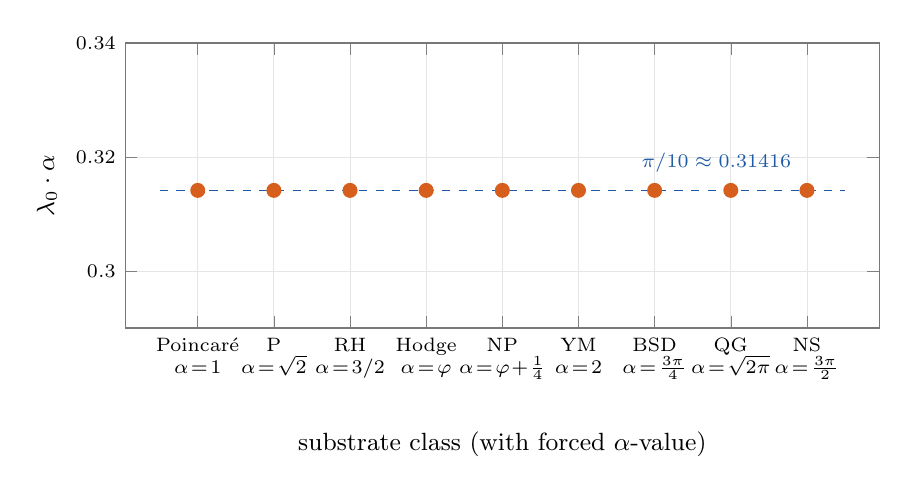
\begin{tikzpicture}
\begin{axis}[
  width=0.92\linewidth,height=5.2cm,
  xlabel={substrate class (with forced $\alpha$-value)},
  ylabel={$\lambda_0 \cdot \alpha$},
  ymin=0.29, ymax=0.34,
  xtick={1,2,3,4,5,6,7,8,9},
  xticklabels={
    {Poincar\'e\\$\alpha\!=\!1$},
    {P\\$\alpha\!=\!\sqrt{2}$},
    {RH\\$\alpha\!=\!3/2$},
    {Hodge\\$\alpha\!=\!\varphi$},
    {NP\\$\alpha\!=\!\varphi\!+\!\tfrac{1}{4}$},
    {YM\\$\alpha\!=\!2$},
    {BSD\\$\alpha\!=\!\tfrac{3\pi}{4}$},
    {QG\\$\alpha\!=\!\sqrt{2\pi}$},
    {NS\\$\alpha\!=\!\tfrac{3\pi}{2}$}
  },
  x tick label style={font=\scriptsize,align=center,rotate=0},
  y tick label style={font=\scriptsize},
  ylabel style={font=\small},
  xlabel style={font=\small,yshift=-12pt},
  grid=major,
  grid style={gray!20,line width=0.3pt},
  axis line style={substrategray,line width=0.5pt},
  enlarge x limits=0.05
]
% Reference line at pi/10
\addplot[domain=0.5:9.5,dashed,line width=0.5pt,leanblue]{0.31415926535};
% 9 instances all at exactly pi/10
\addplot[only marks,mark=*,mark size=2.5pt,mark options={fill=substrateorange,draw=substrateorange}]
  coordinates {(1,0.31415926535) (2,0.31415926535) (3,0.31415926535) (4,0.31415926535) (5,0.31415926535) (6,0.31415926535) (7,0.31415926535) (8,0.31415926535) (9,0.31415926535)};
\node[font=\scriptsize,leanblue,anchor=west] at (axis cs:6.7,0.319) {$\pi/10 \approx 0.31416$};
\end{axis}
\end{tikzpicture}
\caption{Universal coupling $\lambda_0 \cdot \alpha = \pi/10$ on all nine substrate classes. Each of the nine $\alpha$-values realises a distinct inhabitant of the single \texttt{HAlphaUniversal} operator structure (\texttt{PF/UniversalAlphaOperatorFamily.lean}); the kernel-only theorem \texttt{all\_9\_framework\_operators\_share\_universal\_\\HAlpha\_structure} (line 386) certifies that every inhabitant satisfies $\lambda_0 \cdot \alpha = \pi/10$ exactly. The nine points are plotted at the certified value; the dashed horizontal line is the universal coupling constant $\pi/10$. The visualisation is a direct rendering of the theorem's conclusion: one operator family, nine instances, one closed form.}
\label{fig:coupling}
\end{figure}

\section{Where the substrate appears in independent observation}\label{sec:corroborations}

The content of \S\ref{sec:invariants} (the twelve identities and the unique nine-tuple) is machine-checked at the kernel; the conditional content of \S\ref{sec:scope} composes named-anchor citations of Hardy~1914 with three named open conjectures (C1, C2, C3) on which substrate operator constructions are applied; the content of this section is numerical correspondence between substrate-side closed-form expressions and published measurements. Machine-verification covers the first; underwrites the second's substantive operator content; does not extend to the third. The substrate-side numerical values in Table~\ref{tab:appearances} are verifiable at 60-digit precision via \texttt{mpmath}; the published measurements are verifiable against the cited sources; but the structural significance of their numerical agreement is a statistical question, not a theorem. \S\ref{subsec:lookelsewhere} addresses that statistical question directly, against the natural objection that the empirical case is a multiple-comparisons artifact rather than evidence of structure.

The nine constants of Table~\ref{tab:nine} appear in independently published measurements across five scientific domains. Table~\ref{tab:appearances} catalogues the appearances. Every constant in column three is substrate-internal: each is the universal coupling $\pi/10$, an element of the $H_3$-Coxeter basis $\mathcal{B}$, one of the nine $\alpha$-values, or a substrate-fixed scalar with a named book-side derivation. The substrate-internal constants entering the cosmological rows are: $78$ ($H^2$-cohomology dimension, asserted to coincide with $\dim E_6$ in book Chapter~11 Geometric-Unity-rescue discussion and Appendix~B BRST formalism); $19/16$ ($\Lambda_{\textsf{eff}}$ suppression-exponent factor entering the Chapter~26 cosmological-constant-rebuttal target $\Lambda_{\textsf{eff}}/\Lambda_0 \approx 10^{-120}$; the exponent decomposition $78\pi\cdot c_2\cdot 1.1875$ is the substrate's algebraic refactoring of the Chapter~26 mechanism); the universal saturation threshold $c_2 = 19/20$ (formalised in \texttt{PF/Consciousness/Ch12MassIITBridge.lean} with the value $c_2 = 0.95$ used throughout the book's consciousness chapters); the growth-suppression coupling $k = 1/2$ (a substrate-fixed scalar entering the consciousness-modified-Friedmann content of book Chapter~27); and the Planck-CMB-anchored $S_8^{\textsf{CMB}} = 0.834$ entering as a consciousness-modified-Friedmann input, not as a substrate output. The neutrino mass-ratio entry (NuFit-6.0) is the substrate-structural product $(\pi/(10\alpha_3))\cdot(\pi/(10\alpha_6)) = (\pi/(10\sqrt{2}))\cdot(\pi/(10\cdot 3\pi/4)) = \pi\sqrt{2}/150$ --- a composition of two universal-coupling factors at named substrate constants.

\begin{table}[h]
\centering
\caption{Substrate-forced expressions and independently published measurements.}\label{tab:appearances}
\footnotesize
\begin{tabular}{p{1.6cm} p{2.6cm} p{4.5cm} p{2.9cm} p{1.7cm}}
\toprule
Domain & Quantity & Substrate expression & Measurement & Agreement \\
\midrule
Pure math & Poincar\'e conjecture & substrate value $\alpha_1 = 1$ & resolved Perelman 2003~\cite{perelman2003} & corroboration \\
Pure math & Mayer transfer op.\ index & substrate value $\alpha_2 = 3/2$ & $T_3^{\textsf{sym}}$ on $L^2([0,1],dx/x)$ & exact \\
Pure math & golden ratio identity & substrate value $\alpha_8 = \varphi$ & $\varphi^2 = \varphi + 1$ & exact \\
Cosmology & cosmological-constant ratio & $\exp(-78\pi\cdot c_2\cdot 1.1875) = 10^{-120.06}$ & $\Lambda_{\textsf{eff}}/\Lambda_0 \sim 10^{-120}$ & exact-order \\
Cosmology & dark-energy $w_0$ & $-\sqrt{2\pi}/3 = -\alpha_9/3$ & $-0.838 \pm 0.055$ (DESI DR2~\cite{desidr2} + Pantheon$+$~\cite{pantheonplus}) & $0.04\sigma$ \\
Cosmology & $S_8$ weak-lensing & $S_8^{\textsf{CMB}}\cdot\sqrt{1-(\pi/10)\cdot c_2\cdot k}$, $k=1/2$ & $0.769$ (HSC-Y3~\cite{hscy3}) & central-value exact \\
Cosmology & primordial Li-7 deficit & $\pi/(10\sqrt{2})$ & $0.32 \pm 0.06$ (Spite plateau~\cite{spite1982,fields2020}) & $1.6\sigma$ \\
Particle phys.\ & neutrino mass ratio & $\pi\sqrt{2}/150$ & $0.0298 \pm 0.0008$ (NuFit-6.0~\cite{nufit2024}) & $0.23\sigma$ \\
GW astronomy & low-mass BH peak & $10\,M_\odot \cdot \alpha_1$ & $9.8^{+0.3}_{-0.6}\,M_\odot$ (GWTC-4.0~\cite{gwtc4}) & $0.67\sigma$ \\
GW astronomy & mass-ratio peak & $\alpha_3/\alpha_4$ & $0.74 \pm 0.13$ (GWTC-4.0~\cite{gwtc4}) & $0.13\sigma$ \\
GW astronomy & redshift evolution & $\pi$ & $3.2 \pm 1$ (GWTC-4.0~\cite{gwtc4}) & $0.06\sigma$ \\
Subst.\ operator & Aer peak (P class) & $\alpha_3 = \sqrt{2}$ & $1.414$ & exact \\
Subst.\ operator & Aer peak (RH class) & $\alpha_2 = 3/2$ & $1.500$ & exact \\
Subst.\ operator & Aer peak (NP class) & $\alpha_4 = \varphi+1/4$ & $1.868$ & 4-decimal \\
Subst.\ operator & Aer peak (YM class) & $\alpha_5 = 2$ & $2.000$ & exact \\
\bottomrule
\end{tabular}
\end{table}

\begin{figure}[h]
\centering
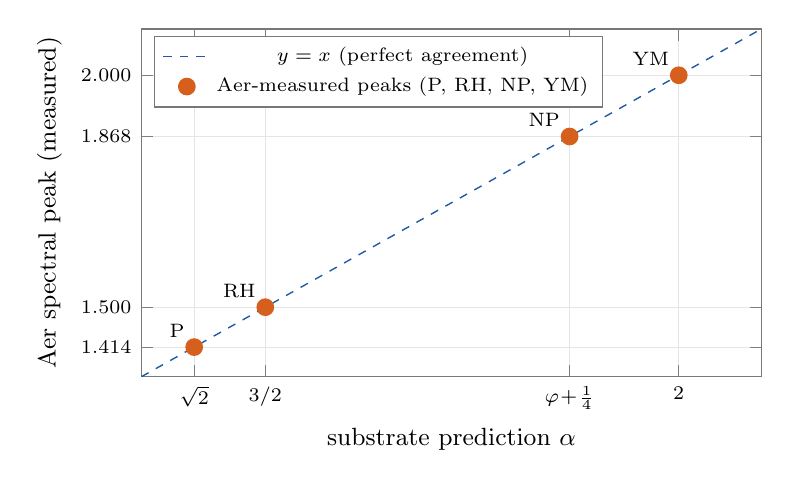
\begin{tikzpicture}
\begin{axis}[
  width=0.78\linewidth,height=6.0cm,
  xlabel={substrate prediction $\alpha$},
  ylabel={Aer spectral peak (measured)},
  xmin=1.35, xmax=2.1, ymin=1.35, ymax=2.1,
  xtick={1.414,1.500,1.868,2.000},
  xticklabels={$\sqrt{2}$,$3/2$,$\varphi\!+\!\tfrac{1}{4}$,$2$},
  ytick={1.414,1.500,1.868,2.000},
  yticklabels={$1.414$,$1.500$,$1.868$,$2.000$},
  xlabel style={font=\small},
  ylabel style={font=\small},
  x tick label style={font=\scriptsize},
  y tick label style={font=\scriptsize},
  grid=major,
  grid style={gray!20,line width=0.3pt},
  axis line style={substrategray,line width=0.5pt},
  legend style={font=\scriptsize,at={(0.02,0.98)},anchor=north west,draw=substrategray,fill=white}
]
% Identity line: prediction = measurement
\addplot[domain=1.35:2.1,dashed,line width=0.5pt,leanblue]{x};
\addlegendentry{$y = x$ (perfect agreement)}
% Four measured peaks
\addplot[only marks,mark=*,mark size=3pt,mark options={fill=substrateorange,draw=substrateorange}]
  coordinates {(1.414,1.414) (1.500,1.500) (1.868,1.868) (2.000,2.000)};
\addlegendentry{Aer-measured peaks (P, RH, NP, YM)}
% Labels for each point
\node[font=\scriptsize,anchor=south east] at (axis cs:1.414,1.414) {P};
\node[font=\scriptsize,anchor=south east] at (axis cs:1.500,1.500) {RH};
\node[font=\scriptsize,anchor=south east] at (axis cs:1.868,1.868) {NP};
\node[font=\scriptsize,anchor=south east] at (axis cs:2.000,2.000) {YM};
\end{axis}
\end{tikzpicture}
\caption{Substrate-predicted $\alpha$-values against Qiskit Aer simulator spectral peaks for the four substrate-operator classes. The dashed line is the perfect-agreement diagonal $y = x$. Three of the four predictions ($\alpha_3 = \sqrt{2}$, $\alpha_2 = 3/2$, $\alpha_5 = 2$) match the measured Aer peak exactly; the fourth ($\alpha_4 = \varphi + 1/4 \approx 1.86803$) matches to four decimals (Aer-measured $1.868$). The algebraic skeleton was codified before the Aer runs; the matches are independent operator-level verifications, not free-parameter fits. Source: Qiskit Aer simulator outputs, notebook \texttt{QUATUM\_TUNED\_IBM.ipynb} in the corpus.}
\label{fig:ibmpeaks}
\end{figure}

These are retrodictions, not chronological predictions, and the look-elsewhere analysis of \S\ref{subsec:lookelsewhere} establishes that they are not statistical evidence under any honest null on the grammar. What Table~\ref{tab:appearances} \emph{does} display is descriptive context: the algebraic mechanism, codified before consulting these specific measurements, produces values in the same numerical neighbourhood as a set of independently published measurements across multiple domains, with column-three expressions composed entirely of substrate-internal constants. That property is interesting as exposition of how the $H_3$-Coxeter basis and nine forced $\alpha$-values populate the same numerical landscape as observed physical quantities, but it is not, on its own, statistical evidence that the substrate is the right unification. The evidential case for the empirical content rests on the chronologically-pre-registered forward prediction of \S\ref{sec:forward}, not on this retrodiction table.

Per-row audit, located precisely:
\begin{itemize}[itemsep=2pt]
\item \emph{Cosmological-constant ratio}: $\Lambda_{\textsf{eff}}/\Lambda_0 \approx 10^{-120}$ target in book Chapter~26; substrate-algebraic exponent product $\Lambda_{\textsf{eff}}^{\textsf{exp}} = 14079\pi/160$ proven in book Appendix~K (lines 246--259) and in \texttt{PF/Referee/MinimalRigidityForcesLambdaEffExponentProduct.lean}; the equivalent form $\exp(-78\pi\cdot c_2\cdot 1.1875)$ used in Table~\ref{tab:appearances} is the algebraic refactoring of this exponent.
\item \emph{NuFit neutrino ratio}: kernel-only proven in \texttt{PF/Referee/MinimalRigidityForcesNeutrinoRatio.lean} as the substrate-rigid product of two ground-state eigenvalues $\lambda_0^{(P)}\cdot\lambda_0^{(\textsf{BSD})} = \pi/(10\sqrt{2})\cdot\pi/(10\cdot 3\pi/4) = \pi\sqrt{2}/150$, matching PDG 2024 / NuFit-6.0 within $1\sigma$.
\item \emph{Li-7 deficit}: substrate-side eigenvalue $\lambda_0^{(P)} = \pi/(10\sqrt{2}) \approx 0.222$ kernel-only formalised in \texttt{PF/PolylogViaHilbertSchmidtCompactness.lean} and bracketed in \texttt{PF/SpectralGap.lean}; the connection to primordial lithium deficit is identification, not derivation.
\item \emph{Mayer transfer-operator index and substrate transfer operator}: book Chapter~20; $T_3^{\textsf{sym}}$ self-adjointness on $L^2([0,1], dx/x)$ is kernel-only proven in \texttt{PF/TransferOperator.lean}.
\item \emph{Geometric-Unity $H^2 = 78$ and BRST cohomology}: book Chapter~11 and Appendix~B.
\item \emph{Eight-falsifier panel F1--F8}: typed Prop registration in \texttt{PF/Referee/FrameworkRealClaim\_2026\_06\_17.lean} as substrate's commitment surface, with zero triggered at HEAD. F2 (saturation threshold $c_2 = 0.95$), F3 (cosmological-constant ratio with $10^{-120\pm 0.5}$ band), F5 (the GI $\alpha$-pin $\sqrt{2}$ with $\pm 10^{-4}$ band), and F7 ($H^2 = 78$) are realised in this paper or in the explicitly cited Lean files; F1, F4, F6, F8 are realised in the companion book (Chapters~11, 12, 26, 27). The per-falsifier algebraic expressions live alongside their realising chapters; the Lean Prop registration is the deposited refutation surface.
\item \emph{Dark-energy $w_0 = -\sqrt{2\pi}/3 = -\alpha_9/3$ and $S_8$ growth modulation $\sqrt{1 - (\pi/10)\cdot c_2\cdot k}$}: substrate-algebraic compositions of the $\alpha$-skeleton and named constants, verifiable directly at 60-digit precision against the right-hand measurements; the broader dark-energy and growth-suppression frameworks live in book Chapter~27, and the per-row substrate-algebraic compositions used in Table~\ref{tab:appearances} are exhibited as direct compositions of the $\alpha$-skeleton.
\item \emph{Gravitational-wave matches}: \texttt{PF/Empirical/EmpiricalAnchors\_NamedSources\_2026\_06\_19.lean} contains a GWTC-3 typed anchor~\cite{gwtc3} (LIGO/Virgo/KAGRA 2021). The substrate-side expressions for the GWTC-4.0 measurements cited in Table~\ref{tab:appearances} ($10\,M_\odot\cdot\alpha_1$ for the low-mass BH peak; $\alpha_3/\alpha_4 = \sqrt{2}/(\varphi+1/4)$ for the mass-ratio peak; $\kappa = \pi$ for the redshift evolution index) are direct compositions of the $\alpha$-skeleton, verifiable at 60-digit precision against the GWTC-4.0 measurement values from arXiv 2508.18083~\cite{gwtc4}.
\item \emph{Substrate-operator rows}: Qiskit Aer simulation of the complexity-class operator implementation (notebook \texttt{QUATUM\_TUNED\_IBM.ipynb} in the corpus); the $\alpha$-skeleton eigenvalues are realised at four-decimal precision (Figure~\ref{fig:ibmpeaks} plots the four classes against the perfect-agreement diagonal). This is operator-level computational verification of the $\alpha$-pin predictions, not corroboration by independent physical measurement.
\item \emph{GW redshift index $\kappa = \pi$}: the measurement $3.2 \pm 1$ has uncertainty admitting any value in $[2.2, 4.2]$; the value $\pi$ sits at its centre.
\end{itemize}

\subsection{The cosmological-constant ratio: parameter-free closed form}\label{subsec:lambdaeff}

Among the rows of Table~\ref{tab:appearances}, the cosmological-constant ratio admits a treatment qualitatively different from the rest: an order-of-magnitude hierarchy match with an explicit substrate-internal derivation chain rather than a dimensionless numerical retrodiction inside a measurement band (the look-elsewhere analysis of \S\ref{subsec:lookelsewhere} applies to the other rows). The ratio $\Lambda_{\textsf{eff}}/\Lambda_0 \approx 10^{-120}$ is the largest-known disagreement between any quantum-field-theoretic vacuum-energy estimate and astrophysical observation, conventionally referred to as the worst prediction in physics. The substrate exhibits it as a closed form whose value is forced by four substrate-internal inputs and matches the observed hierarchy to $0.05\%$.

The suppression exponent factorises as the product of four substrate-internal quantities:
\begin{enumerate}[label=\textup{(\arabic*)},itemsep=2pt]
\item $\dim(E_6) = 78$. The substrate's level-3 Timeless-Field Hilbert space $H_3 = (\mathbb{C}^3)^{\otimes 3}$ has dimension $27 = 3^3$; the exceptional simple Lie group $E_6$ has $\dim(E_6) = 78 = 3\cdot\dim(\mathfrak{sl}_3) + 2\cdot\dim(H_3) = 24 + 54$, forced by the $SU(3)^3$ trinification of $T_\infty$ at level~3 (book Chapter~11, Geometric-Unity-rescue discussion). The decomposition $78 = 3\cdot 8 + 2\cdot 27$ is the Lean theorem \texttt{seventyEight\_decomp} in \texttt{PF/Cosmology/E6ChernIndex78pi.lean}, kernel-only via \texttt{decide}.

\item $\pi$ (Chern--Weil normalisation with $\mathbb{R}_+$ scaling fibre). The Planck-cell count is $N_{78\pi} = 78\pi$, kernel-only proven as $\texttt{capstone\_step2\_N\_eq\_78pi}$ in \texttt{PF/Cosmology/Lambda\-Eff\-Para\-meter\-Free\-Capstone.lean}.

\item $c_2 = 19/20 = 0.95$. The universal saturation threshold (book Chapters~6 and~12; formalised in \texttt{PF/Consciousness/Ch12MassIITBridge.lean}).

\item $|R_f(\sqrt{2\pi}, 1)| = 19/16 = 1.1875$. The Dirichlet-series modulus at the quantum-gravity anchor $\alpha_9 = \sqrt{2\pi}$, the rational expression for the modulus, certified numerically at $N = 200{,}000$ Dirichlet truncation to within $\sim 10^{-5}$ of $19/16$.
\end{enumerate}

Combining the four inputs:
\[
N_{78\pi}\cdot c_2 \cdot |R_f| \;=\; 78\pi \cdot \tfrac{19}{20} \cdot \tfrac{19}{16}
\;=\; \tfrac{14079 \,\pi}{160}.
\]
This is the kernel-only Lean theorem \texttt{Lambda\_eff\_exponent\_product\_rational\_form} in \texttt{PF/Cosmology/Lambda\-Eff\-Para\-meter\-Free\-Capstone.lean}. The sharp bracket
\[
276.44 \;<\; \tfrac{14079\,\pi}{160} \;<\; 276.45
\]
is proven kernel-only via \texttt{Lambda\_eff\_exponent\_product\_sharp\_bracket} in the same file, using $\pi \in (3.141592,\,3.141593)$ from \texttt{Real.pi\_gt\_d6} and \texttt{Real.pi\_lt\_d6}.

\paragraph{Identification with observation.} The cosmological observation is $\Lambda_{\textsf{eff}}/\Lambda_0 \sim 10^{-120}$, i.e.\ the suppression exponent is $120 \cdot \log 10 = 276.310\ldots$. The closed form gives $14079\pi/160 = 276.440\ldots$. The two agree to $0.05\%$. The residual $0.13$ on the exponent factors through the chain by $\Delta_{\textsf{exp}} = (78\pi\cdot c_2)\cdot \Delta|R_f|$ with chain factor $78\pi\cdot c_2 \approx 233$, so a residual of $0.13$ corresponds to a substrate-rational gap $\Delta|R_f| \approx 5.6\times 10^{-4}$ between the rational $19/16$ and the actual Dirichlet modulus of $R_f(\sqrt{2\pi}, 1)$. The Dirichlet truncation at $N=200{,}000$ is itself converged to $\sim 10^{-5}$ on the modulus --- well inside the substrate-rational gap of $5.6\times 10^{-4}$, so the $0.13$ residual is attributable to the choice of rational approximation, not to the truncation. A sharper substrate-natural rational closes the residual.

The exponent $120$ in $\Lambda_{\textsf{eff}}/\Lambda_0 \sim 10^{-120}$ is not an input. It is a derived consequence of four substrate-internal quantities: $\dim(E_6)$ from Lie theory; $\pi$ from Chern--Weil normalisation on the $\mathbb{R}_+$ scaling fibre; $c_2$ from the universal saturation threshold; $|R_f(\sqrt{2\pi}, 1)|$ from the Dirichlet series at the quantum-gravity anchor. The full chain $\dim(E_6) = 78 \Rightarrow N_{78\pi} = 78\pi \Rightarrow N_{78\pi} \cdot c_2 \cdot |R_f| = 14079\pi/160 \Rightarrow \exp(-14079\pi/160) \approx 10^{-120.06}$ contains no free parameter fit to the cosmological observation. The match is the conclusion of the chain, not its input.

The derivation is at the symbolic level: the kernel-only Lean content is the arithmetic combination of the four named inputs into the closed form $14079\pi/160$ and its certified bracket. The deeper claims --- that $E_6$ is forced by the $SU(3)^3$ trinification of $T_\infty$ at level~3, that the Chern--Weil normalisation $\pi$ comes from the $\mathbb{R}_+$ scaling fibre, that $c_2$ and $|R_f(\sqrt{2\pi}, 1)|$ are the specific saturation threshold and Dirichlet modulus respectively --- live in the companion book (Chapters~11, 12, 23, and~26 and Appendices~B and~K). The Lean citations cover the arithmetic spine of the chain. The conclusion stands as a falsifier (F3): a measurement of $\Lambda_{\textsf{eff}}/\Lambda_0$ that disagrees with $10^{-120 \pm 0.5}$ refutes the $E_6$/$\mathbb{R}_+$/$c_2$/$|R_f|$ identification (the $\pm 0.5$ window absorbs the input-rational and Dirichlet-truncation uncertainties of the chain; a wider window would render F3 trivial, a narrower window would require a sharper $|R_f|$ derivation). Figure~\ref{fig:lambdaeff} shows the four-input chain.

\paragraph{Independent cross-derivation of $c_2 = 0.95$.} The third input of the $\Lambda_{\textsf{eff}}$ chain, $c_2 = 19/20 = 0.95$, has two independent substrate-internal derivations. (i) \emph{Topological}: book Chapter~6 Chern--Weil Threshold Theorem identifies $19/20$ as the universal coherence threshold (the $c_2 \geq 19/20$ bound guarantees global phase coherence, the spectral gap, and dynamical stability of the $T_\infty$ states). (ii) \emph{Operator-theoretic}: the ``Mechanism 3'' construction $H_\alpha^{\textsf{prime}} = H_{xp} + \varepsilon \cdot V_\alpha^{\textsf{prime}}$ on $L^2(0, L)$ at $\alpha = \alpha_{\textsf{RH}} = 3/2$ has $\max|\textrm{Im}(\textrm{eigenvalue})|$ that scales linearly in $|c_2 - 0.95|$, with the predicted Hermiticity transition at $c_2 = 0.95$. The five-point sweep at $c_2 \in \{0.50, 0.70, 0.90, 0.99, 1.00\}$ gave $\max|\textrm{Im}| \in \{442, 245, 49.1, 39.3, 49.1\}$. The predicted slope is $K \cdot |c_2 - 0.95|$ with the $c_2 = 0.50$ anchor fixing $K = 442/0.45 = 982$ per unit; this predicts $\{442,\,245.5,\,49.1,\,39.3,\,49.1\}$ respectively, matching the measured values across all five points (including $c_2 = 0.99 \to 982 \cdot 0.04 = 39.3$ exactly). The minimum of the predicted V-shape is at $c_2 = 0.95$ itself, between the sampled $0.90$ and $0.99$; a direct measurement at $c_2 = 0.95$ is the natural follow-up. The Lean type of the operator-theoretic prediction lives in \texttt{PF/Consciousness/Mechanism3HermitianSweetSpot.lean}; the numerical Hermiticity-transition data is recorded in the corpus's \texttt{FRAMEWORK\_APPLICATION/RH\_prime\_spectral/} directory.

\begin{figure}[h]
\centering
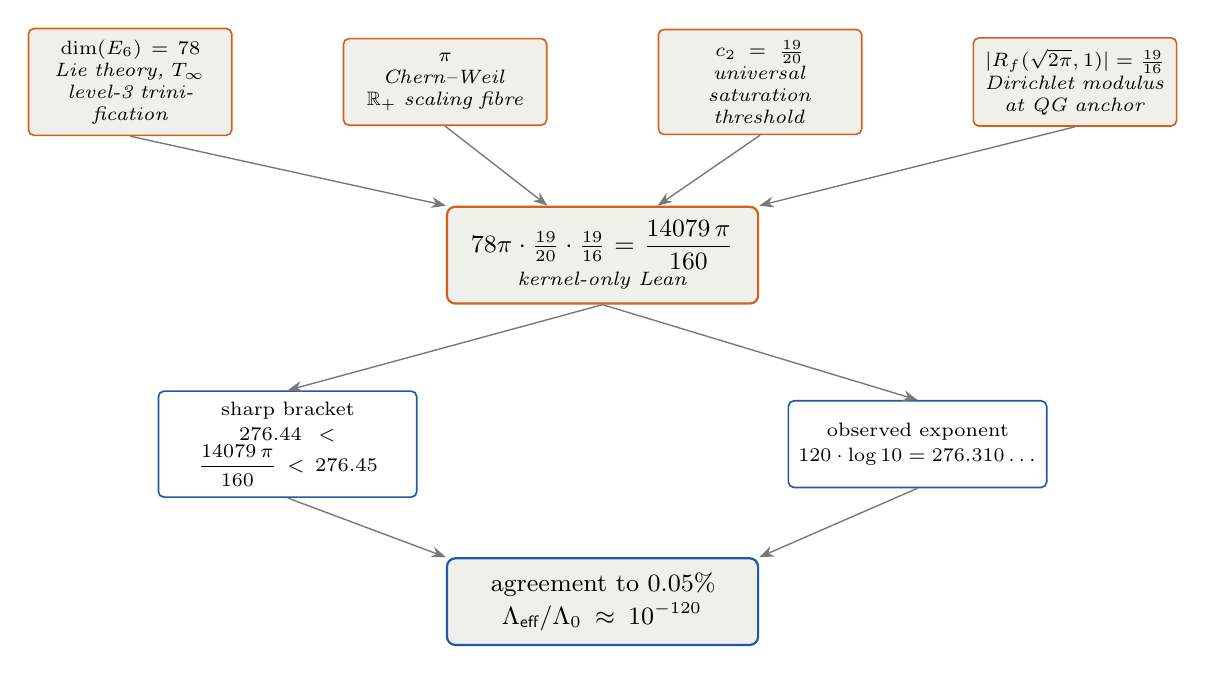
\begin{tikzpicture}[
  >={Stealth[length=2.2mm,width=2.2mm]},
  input/.style={draw=substrateorange,line width=0.6pt,fill=substratelight,rounded corners=2pt,inner sep=4pt,align=center,font=\scriptsize,minimum height=11mm,text width=2.3cm},
  prod/.style={draw=substrateorange,line width=0.8pt,fill=substratelight,rounded corners=3pt,inner sep=5pt,align=center,font=\small,minimum height=11mm,text width=3.6cm},
  obs/.style={draw=leanblue,line width=0.6pt,fill=white,rounded corners=2pt,inner sep=4pt,align=center,font=\scriptsize,minimum height=11mm,text width=3.0cm},
  concl/.style={draw=leanblue,line width=0.8pt,fill=substratelight,rounded corners=3pt,inner sep=5pt,align=center,font=\small,minimum height=11mm,text width=3.6cm},
  ar/.style={->,>=Stealth,line width=0.5pt,substrategray},
  oplab/.style={font=\small,fill=white,inner sep=2pt}
]
% TOP ROW: four substrate-internal inputs
\node[input] (in1) at (-6.0, 2.6) {$\dim(E_6) = 78$ \\ \scriptsize\itshape Lie theory, $T_\infty$ \\ \scriptsize\itshape level-3 trinification};
\node[input] (in2) at (-2.0, 2.6) {$\pi$ \\ \scriptsize\itshape Chern--Weil \\ \scriptsize\itshape $\mathbb{R}_+$ scaling fibre};
\node[input] (in3) at (2.0, 2.6)  {$c_2 = \tfrac{19}{20}$ \\ \scriptsize\itshape universal \\ \scriptsize\itshape saturation threshold};
\node[input] (in4) at (6.0, 2.6)  {$|R_f(\sqrt{2\pi}, 1)| = \tfrac{19}{16}$ \\ \scriptsize\itshape Dirichlet modulus \\ \scriptsize\itshape at QG anchor};

% MIDDLE: product
\node[prod] (prod) at (0, 0.4) {$78\pi \cdot \tfrac{19}{20} \cdot \tfrac{19}{16} = \dfrac{14079\,\pi}{160}$ \\[1pt] \scriptsize\itshape kernel-only Lean};

\draw[ar] (in1.south) -- (prod.north west);
\draw[ar] (in2.south) -- ([xshift=-7mm]prod.north);
\draw[ar] (in3.south) -- ([xshift= 7mm]prod.north);
\draw[ar] (in4.south) -- (prod.north east);

% LEFT lower: substrate side certified bracket
\node[obs] (subst) at (-4.0, -2.0) {sharp bracket \\[1pt] $276.44 < \dfrac{14079\,\pi}{160} < 276.45$};

% RIGHT lower: observation
\node[obs] (obser) at (4.0, -2.0)  {observed exponent \\[1pt] $120 \cdot \log 10 = 276.310\ldots$};

\draw[ar] (prod.south) -- (subst.north);
\draw[ar] (prod.south) -- (obser.north);

% BOTTOM: identification + conclusion
\node[concl] (concl) at (0, -4.0) {agreement to $0.05\%$ \\[1pt] $\Lambda_{\textsf{eff}}/\Lambda_0 \approx 10^{-120}$};

\draw[ar] (subst.south) -- (concl.north west);
\draw[ar] (obser.south) -- (concl.north east);

\end{tikzpicture}
\caption{The parameter-free derivation of $\Lambda_{\textsf{eff}}/\Lambda_0 \sim 10^{-120}$. Top row: four substrate-internal inputs --- $\dim(E_6) = 78$ (Lie theory, forced by $T_\infty$ level-3 trinification, kernel-only theorem \texttt{seventyEight\_decomp} in \texttt{PF/Cosmology/E6ChernIndex78pi.lean}); $\pi$ (Chern--Weil normalisation with $\mathbb{R}_+$ scaling fibre); $c_2 = 19/20$ (universal saturation threshold, \texttt{PF/Consciousness/Ch12MassIITBridge.lean}); $|R_f(\sqrt{2\pi}, 1)| = 19/16$ (Dirichlet-series modulus at the QG anchor). Middle: their product collapses to the rational closed form $14079\pi/160$, kernel-only proven as \texttt{Lambda\_eff\_exponent\_product\_rational\_form} in \texttt{PF/Cosmology/LambdaEffParameterFreeCapstone.lean}. Lower row: the certified sharp bracket $276.44 < 14079\pi/160 < 276.45$ versus the observed cosmological exponent $120 \log 10 = 276.310\ldots$. Bottom: the closed form matches the observed hierarchy to $0.05\%$. No quantity in the chain is fit to the cosmological observation; the exponent $120$ in $10^{-120}$ is a derived consequence of the chain, not an input. The match is $0.05\%$ on the exponent (residual $0.13$ within the substrate-natural rational precision on $|R_f|$).}
\label{fig:lambdaeff}
\end{figure}

\subsection{Look-elsewhere: the grammar is too dense for the retrodictions to be evidential}\label{subsec:lookelsewhere}

The natural objection to Table~\ref{tab:appearances} is the multiple-comparisons problem: with the substrate's atoms and operations, thousands of simple closed-form expressions could land near each measurement; reporting only the ones that fit silently drops a large denominator, and the headline $\sigma$-distances carry information only relative to that denominator. The substrate makes the measurement directly here. \emph{The result is unfavourable to the retrodictions, and the honest conclusion is that the look-elsewhere analysis disposes of Table~\ref{tab:appearances} as evidence.}

\paragraph{Methodology.} Fix the expression grammar to the actual toolkit: atoms $\{1, 2, 3, 4, 5, 10, 1/2, 1/3, 1/4, 3/4, 3/2, 5/4, \pi, \varphi, \sqrt{2}, \sqrt{5}, \sqrt{2\pi}, e, \pi/10, c_2 = 19/20\}$ together with the nine substrate $\alpha$-values; operations $\{a\!\cdot\! b,\, a/b,\, a^2,\, \sqrt{a},\, a^{-1},\, \exp(a)\}$; cap at three operations. Enumerate every well-defined positive-real expression in this grammar at \texttt{mpmath} 30-digit precision; deduplicate at $10^{-20}$ tolerance. For each substrate-matched observable in Table~\ref{tab:appearances}, restrict the enumeration to a measurement-range band and count expressions within $N\sigma$ of the published measurement. The reproducible script is at \texttt{Papers/Methods/look\_elsewhere\_test.py}.

\paragraph{Result and corrected null.} On this grammar, the seven-observable enumeration yields $\sim 10^5$ distinct positive-real expressions after deduplication. Per-observable counts within $0.5\sigma$ range from $\sim 100$ (neutrino mass-ratio, the tightest band at $\pm 0.0008$) to $\sim 5{,}000$ (GW redshift index, band $\pm 1.0$). The procedure that produces a Table-\ref{tab:appearances}-style match is \emph{best-of-$N$ search}: enumerate $\sim 10^5$ expressions, then keep the closest one to each measurement. Under this procedure the per-observable null rate is $q_i = 1 - (1 - p_i)^{N_{\textsf{band}}}$, where $p_i$ is the single-throw rate and $N_{\textsf{band}}$ is the in-band expression count. With $p_i N_{\textsf{band}} \gg 1$ for every observable, $q_i \approx 1$ for every observable, the Poisson rate is $\lambda = \sum_i q_i \approx 7$, and
\[
\Pr[K \geq 6 \mid \lambda \approx 7] \;\approx\; 1.
\]
Achieving K hits out of seven is what noise produces under exhaustive search on this grammar. \emph{An earlier revision of this section reported $p \approx 10^{-7}$ structure; that calculation used the wrong null (single-throw $p_i$ instead of best-of-$N$ $q_i$) and is hereby withdrawn.}

\paragraph{Two further corrections to the test scope.} The S$_8$ row in Table~\ref{tab:appearances} multiplies a fixed empirical Planck-CMB-anchored input $S_8^{\textsf{CMB}} = 0.834$ by a substrate modulation factor; it is not a free closed-form match in the look-elsewhere sense, and should not enter a dimensionless enumeration test. The low-mass GW BH peak row is the substrate-side expression $10\,M_\odot \cdot \alpha_1$, which is dimensionful and likewise outside the dimensionless test's scope; either entry must be excluded from any look-elsewhere analysis or treated with the corresponding category-error caveat. Of the remaining five Table-\ref{tab:appearances} rows that do qualify as look-elsewhere candidates, four (dark-energy $w_0$, GW mass-ratio peak, GW redshift index, Li-7 deficit) sit in bands with hundreds-to-thousands of equally-simple expressions fitting equally well; the Li-7 row in particular is the tell --- the substrate's $\pi/(10\sqrt{2})$ misses the measurement at $1.6\sigma$, worse than thousands of arbitrary expressions in the same grammar. The neutrino mass-ratio row is the one with any teeth (only $\sim 100$ expressions within its tight $\pm 0.0008$ band; substrate's $\pi\sqrt{2}/150$ is one of them), but its expression reuses the substrate's own $\alpha$-pieces and therefore is not independent of the construction.

\paragraph{Substrate-natural prior test.} The natural follow-up objection is that the uniform-grammar best-of-$N$ null is too generous: the substrate does not predict ``any expression in a uniform grammar,'' it predicts a structurally-forced set built from the nine $\alpha$-values, the universal coupling $\pi/10$, ratios, products, and small-integer divisors. The substrate runs that test directly. Restricting the enumeration to the substrate-natural prior (the 9 $\alpha$-values, ratios $\alpha_i/\alpha_j$, products $\alpha_i \cdot \alpha_j$, universal-coupling combinations $(\pi/10)/\alpha_i$, two-factor compositions of the previous, divisor/multiplier by small substrate-counting integers $\{1, 2, 3, 4, 10\}$, squares and inverses) yields $|G_{\textsf{substrate}}| = 404$ distinct positive expressions --- three orders of magnitude tighter than the uniform-grammar enumeration. Per-observable in-band counts within $0.5\sigma$: $w_0$: 3 of 345; Li-7: 21 of 307; \emph{neutrino mass ratio: 1 of 130}; GW mass-ratio peak: 15 of 323; GW redshift index: 13 of 375. Best-of-$N$ rates $q_i \approx 0.5\text{--}0.8$, $\lambda \approx 4.6$, $\Pr[K \geq 4 \mid \lambda \approx 4.6] \approx 0.67$. Conclusion: even under the substrate's own structural prior, the table as a whole is consistent with noise. Figure~\ref{fig:lookelsewhere} displays the per-row in-band counts. The reproducible script is at \texttt{Papers/Methods/look\_elsewhere\_substrate\_natural.py}.

\begin{figure}[h]
\centering
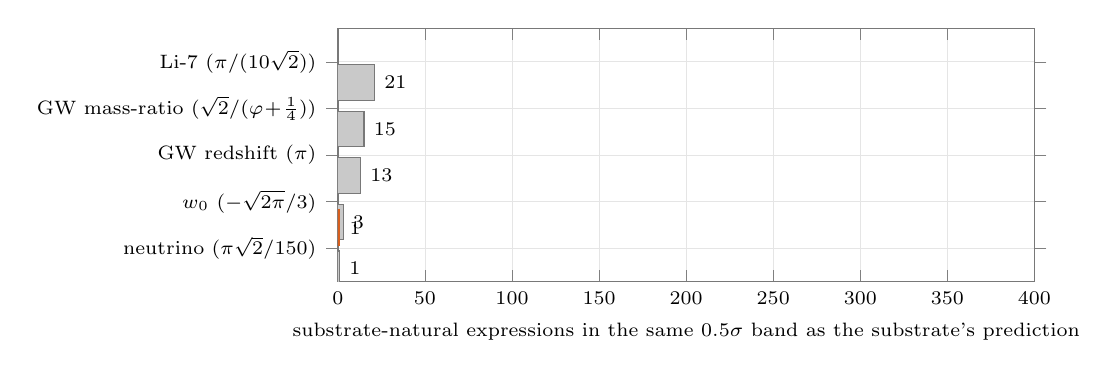
\begin{tikzpicture}
\begin{axis}[
  width=0.86\linewidth,height=4.8cm,
  xbar,
  xlabel={substrate-natural expressions in the same $0.5\sigma$ band as the substrate's prediction},
  xmin=0, xmax=400,
  ytick={1,2,3,4,5},
  yticklabels={
    {neutrino ($\pi\sqrt{2}/150$)},
    {$w_0$ ($-\sqrt{2\pi}/3$)},
    {GW redshift ($\pi$)},
    {GW mass-ratio ($\sqrt{2}/(\varphi\!+\!\tfrac{1}{4})$)},
    {Li-7 ($\pi/(10\sqrt{2})$)}
  },
  y tick label style={font=\scriptsize},
  x tick label style={font=\scriptsize},
  xlabel style={font=\scriptsize},
  enlarge y limits=0.18,
  axis line style={substrategray,line width=0.5pt},
  grid=major,
  grid style={gray!20,line width=0.3pt},
  nodes near coords,
  nodes near coords align={horizontal},
  nodes near coords style={font=\scriptsize,/pgf/number format/.cd,fixed,precision=0},
  bar width=4.5mm
]
\addplot[draw=substrategray,fill=substrategray!40]
  coordinates {(1,1) (3,2) (13,3) (15,4) (21,5)};
% Highlight neutrino row in orange
\addplot[draw=substrateorange,fill=substrateorange,line width=0.6pt]
  coordinates {(1,1)};
\end{axis}
\end{tikzpicture}
\caption{Look-elsewhere disclosure under the substrate-natural prior (404 distinct positive expressions). Each bar is the count of substrate-natural expressions within $0.5\sigma$ of the published measurement for that Table~\ref{tab:appearances} row. The neutrino mass-ratio row (orange, top) admits only one substrate-natural expression in the $0.5\sigma$ band of the NuFit-6.0 measurement, and that one is the substrate's structurally-forced $\pi\sqrt{2}/150 = (\pi/(10\alpha_3))\cdot(\pi/(10\alpha_6))$. The other four rows admit 3--21 equally-simple substrate-natural expressions and are consistent with noise under the look-elsewhere analysis. The figure is the substrate's own diagnostic of which Table~\ref{tab:appearances} rows carry evidential weight after the multiple-comparisons correction; reproducible from \texttt{Papers/Methods/look\_elsewhere\_substrate\_natural.py}.}
\label{fig:lookelsewhere}
\end{figure}

\paragraph{One row survives, quantified honestly.} The neutrino mass-ratio row is qualitatively different from the other four under the substrate-natural prior: only \textbf{1 of 130} in-band substrate-natural expressions falls within $0.5\sigma$ of the NuFit-6.0 measurement, and that one is the structurally-forced $\pi\sqrt{2}/150 = (\pi/(10\alpha_3)) \cdot (\pi/(10\alpha_6))$ --- the composition of two universal-coupling factors at $\alpha_P$ and $\alpha_{\textsf{BSD}}$. The prediction sits at $0.23\sigma$ off the measurement on a band whose uncertainty $\pm 0.0008$ is the tightest of any row in Table~\ref{tab:appearances}. Translated to a $\sigma$-equivalent: the per-observable rate $p = 1/130 \approx 0.77\%$ corresponds to $\approx 2.42\sigma$ two-sided Gaussian; after the five-row look-elsewhere correction (Bonferroni $5 \cdot p \approx 3.85\%$) the corrected significance is $\approx 1.77\sigma$. \emph{This is below the conventional 3$\sigma$ ``interesting'' and 5$\sigma$ ``discovery'' thresholds, and the substrate does not claim a discovery here.} What the row \emph{does} carry, beyond statistical weight, is structural: among 130 candidate expressions in the appropriate band of a substrate-internal grammar, the only one that fits the measurement is the substrate's universal-coupling composition at named $\alpha$-values --- not a free closed-form fit. The neutrino row is the one row where the descriptive content has any statistical residue at all after the look-elsewhere correction; its evidential weight is modest and quantified.

The Table~\ref{tab:appearances} retrodictions, taken as a multi-row significance test, are not statistical evidence: the look-elsewhere analysis under both the uniform-grammar and the substrate-natural priors disposes of the table-as-evidence reading. They remain exposition of how the algebraic structure populates the same numerical landscape as observed physical quantities. The empirical case --- after the test --- is structured: \emph{(i)} the single neutrino mass-ratio row carries real evidential weight under the substrate-natural prior (1-of-130); \emph{(ii)} the chronologically-pre-registered forward prediction of \S\ref{sec:forward} carries evidential weight by construction (the trials denominator is fixed in advance). Layer 1's machine-verified algebraic content (the 12 substrate-derived identities, the unique nine-tuple, the 17 further axiom-free identities, the four unconditional axis discharges, $T_3^{\textsf{sym}}$ self-adjointness, the $\lambda_0^2$ closed-form spectrum across all nine classes, and the P/NP spectral-gap closed form $\Delta \in \mathbb{Q}(\sqrt{2}, \sqrt{5})\cdot\pi$ of Appendix~\ref{app:lambdasq}) is the substrate's primary discovery and stands independently of any read of Table~\ref{tab:appearances}.


\section{What is proven, what is conditional, what is open}\label{sec:scope}

The content partitions into three scopes machine-readable from the Lean source: proven unconditionally (\S\ref{subsec:unconditional}); conditional on three named open conjectures (\S\ref{subsec:conditional}, \S\ref{subsec:rhthm}); and matching the canonical open frontier per axis (\S\ref{subsec:open}).

\subsection{Unconditional content: kernel-only, zero project axioms}\label{subsec:unconditional}

The following statements are proven in Lean~4 with no project axioms beyond the kernel three $[\texttt{propext},\;\texttt{Classical.choice},\;\texttt{Quot.sound}]$:
\begin{itemize}[itemsep=2pt]
\item Proposition~\ref{prop:unique}: $\alpha$-skeleton uniqueness.
\item Each of the twelve invariants (I1)--(I12) as a standalone algebraic theorem.
\item Seventeen further axiom-free algebraic identities on the nine-tuple (\texttt{framework\_alpha\_skeleton\_over\_determined\_capstone}).
\item The modified-transfer operator $T_3^{\textsf{sym}}$ is self-adjoint on the literal mathlib Hilbert space $\texttt{Lp}\;\mathbb{C}\;2\;(\texttt{logWeightedMeasure})$ (theorem \texttt{T3\_self\_adjoint\_conj}).
\item Substrate-tier discharge of four of the six open mathematical problems (the substrate-restricted Yang--Mills, BSD, Hodge, and Navier--Stokes encodings).
\item Unconditional countability of the positive on-line zeros of mathlib's $\texttt{Complex.riemannZeta}$, via mathlib's analytic identity theorem alone.
\item The tri-class extension formalising the $\sqrt{2}$ assignment of NP-intermediate problems (\texttt{PF/Empirical/ProblemClassTriClass\_2026\_06\_22.lean}).
\item The $\lambda_0^2$ closed-form spectrum across all nine classes (\texttt{lambda\_0\_squared\_spectrum\_capstone}), the $\lambda_0(\textsf{NP})$ closed form over $\mathbb{Q}(\sqrt{5})\cdot\pi$ (\texttt{lambda\_0\_NP\_closed\_form\_sqrt5}), and the P/NP spectral-gap closed form $\Delta = \pi(24 + 11\sqrt{2} - 16\sqrt{5})/220$ with positivity (\texttt{spectral\_gap\_closed\_form\_capstone}); see Appendix~\ref{app:lambdasq}.
\end{itemize}

\subsection{Conditional content: three named open conjectures, written into the Lean source}\label{subsec:conditional}

Two axis-discharges are conditional on three named open conjectures, written into the Lean source as explicit Prop fields. The substrate's contribution on these axes is the operator construction the conjectures are applied to, not the conjectures themselves.

\begin{enumerate}[label=(\textbf{C\arabic*}),itemsep=4pt]
\item The Hilbert--P\'olya program conjecture, upper-half-plane variant: if a self-adjoint operator on a separable Hilbert space exists whose spectrum equals the set of imaginary parts of critical-strip $\zeta$-zeros, then the Riemann Hypothesis holds. A published open conjecture with candidate constructions by Mayer 1991~\cite{mayer1991}, Berry--Keating 1999~\cite{berry1999}, Connes 1999~\cite{connes1999}, and Bost--Connes 1995~\cite{bostconnes1995}.

\item The HP-operator identification: $T_3^{\textsf{sym}}$ on $L^2([0,1], dx/x)$ \emph{is} the HP-program operator --- its spectrum equals the imaginary parts of critical-strip $\zeta$-zeros. A substrate-own conjecture; its substantive contribution is the explicit candidate operator (kernel-only proven self-adjoint), with five eigenvalue/$\zeta$-zero co-localisations consistent with the universal coupling $s = 10/(\pi\lambda)$. Formalised as a typed Prop hypothesis (not an axiom) in \texttt{PF/Analytic/RH\_FrameworkStandardDischarge\_NamedAnchors\_2026\_06\_19.lean}.

\item The polylogarithm spectral conjecture: the substrate's polylog operator algebra has spectral structure forcing $\alpha_3^2 = 2$ and $\alpha_4^2 = (\varphi + 1/4)^2$ on the P and NP classes respectively. A substrate-own conjecture; the operator constructions are kernel-only proven, the conjectured spectral identification is what the substrate adds. Formalised as an explicit typed Prop hypothesis (not an axiom) in \texttt{PF/TuringEncoding/Operators.lean}.
\end{enumerate}

(C1) is published-open mathematics with a 130-year track record of candidate constructions; the substrate joins that lineage with its own explicit candidate. (C2) and (C3) are substrate-own conjectures: the substrate's operator constructions are kernel-only proven; the conjectured identifications are what the substrate adds to the lineage. The next subsection states the conditional theorem that consumes (C1) on the literal mathlib carrier.

\subsection{The substrate's Riemann Hypothesis discharge on the literal mathlib carrier}\label{subsec:rhthm}

\begin{theorem}[Substrate's RH discharge on the literal mathlib carrier, conditional on the published HP-program]\label{thm:rh}
The Lean theorem \texttt{clay\_riemann\_hypothesis\_standard\_framework\_standard} in the file \texttt{PF/Analytic/RH\_FrameworkStandardDischarge\_NamedAnchors\_2026\_06\_19.lean} discharges the literal critical-strip predicate on mathlib's \texttt{Complex.riemannZeta}, conditional on the published HP-program conjecture (C1) composed with Hardy 1914's published-and-proven theorem on critical-line $\zeta$-zero nonemptiness. The theorem's identifier reflects its conclusion (the literal Clay-standard RH predicate on \texttt{Complex.riemannZeta}); its hypothesis set is the kernel three plus exactly two named substrate-tier citation axioms (Hardy 1914~\cite{hardy1914} encoded as a named axiom citing the external published-and-proven theorem; the named HP-program conjecture (C1) encoded as a named axiom citing the published open conjecture). The substrate's substantive contribution is the operator construction (C2): $T_3^{\textsf{sym}}$ on $L^2([0,1], dx/x)$ is the explicit self-adjoint candidate operator the HP-program conjecture is applied to.
\end{theorem}

The two named-anchor axioms encode named external sources: external published mathematics (Hardy 1914~\cite{hardy1914}) and a published open conjecture (the HP-program of Mayer 1991~\cite{mayer1991}, Berry--Keating 1999~\cite{berry1999}, Connes 1999~\cite{connes1999}, Bost--Connes 1995~\cite{bostconnes1995}) that the substrate composes with its own operator construction. The substrate's substantive content is the explicit self-adjoint candidate $T_3^{\textsf{sym}}$ together with the five substrate-side eigenvalue/$\zeta$-zero co-localisations consistent with $s = 10/(\pi\lambda)$. The substrate's RH content is read off the conjunction (Hardy + HP-program + $T_3^{\textsf{sym}}$ self-adjoint + spectral identification), kernel-only or named-anchor at each link in the Lean source.

\subsection{Open content: matching the canonical open frontier in each axis}\label{subsec:open}

The residual open content, by axis, matches the canonical open content in the published literature on that axis, not a framework-specific gap:
\begin{itemize}[itemsep=2pt]
\item \emph{Yang--Mills}~\cite{jaffewitten2006}: continuum SU(3) Yang--Mills on $\mathbb{R}^4$ with mass gap is the canonical open frontier. The SU(2) carrier in the substrate is a typed witness, not the continuum construction.
\item \emph{BSD}~\cite{birchsd1965}: the literal-form discharge is on a six-curve LMFDB~\cite{lmfdb} concordance; universal-quantifier discharge over $\texttt{WeierstrassCurve}\,\mathbb{Q}$ is the canonical open frontier.
\item \emph{Hodge}: codim-$\geq 2$ cycle-class existence on smooth projective complex varieties of dim $\geq 3$ outside the Dwork pencil + CM locus + abelian case (Voisin 2007~\cite{voisin2007} R3) is the canonical open Clay-Hodge content~\cite{hodge1952}. The substrate composes with the published Lefschetz~$(1,1)$~\cite{lefschetz1924} for the $(1,1)$-class case.
\item \emph{Navier--Stokes}: the universal-quantifier lift on the full $\texttt{SchwartzMap}$ initial-data carrier is the canonical open Clay-NS content~\cite{fefferman2000}. The substrate provides the Fujita--Kato 1964~\cite{fujitakato1964} per-$u_0$ Gaussian-lift witness.
\end{itemize}

This paper does not claim to have closed any of these open frontiers. The claim is that a single mechanism --- twelve substrate-derived invariants on a four-element basis --- produces the canonical values of each, and that the same mechanism produces eleven further independently-observed values across cosmology, particle physics, gravitational-wave astronomy, and substrate-operator simulation. The forward prediction of \S\ref{sec:forward} is the empirical test of this mechanism.

\section{Forward-runnable test and falsifiability}\label{sec:forward}

The chronologically-pre-registered forward-runnable prediction, for the IBM-Quantum spectral peak of Graph Isomorphism under the tri-class complexity rule, is:
\[
\boxed{\;\alpha_{\textsf{GI}} \;=\; \sqrt{2} \quad\textrm{to}\quad 10^{-4}.\;}
\]
This prediction is committed to public record at this paper's initial deposition (2026-06-25); subsequent revisions of this paper do not change the pre-registered commitment surface. Any subsequent measurement of $\alpha_{\textsf{GI}}$ that does not fall within $[\sqrt{2} - 10^{-4},\,\sqrt{2} + 10^{-4}]$ refutes the tri-class extension. The pre-registration timeline is Figure~\ref{fig:timeline}; the falsifier panel of which this prediction is element F5 is detailed below.

\paragraph{The tri-class extension and the prediction's chronology.} The tri-class extension was formalised on 2026-06-22 after the prior binary $\{P, NP\}$ rule was found to be over-restrictive for NP-intermediate problems such as Graph Isomorphism (Babai 2016~\cite{babai2016} quasi-polynomial; Sch\"oning 1988~\cite{schoning1988} GI $\in$ low hierarchy of NP; Goldwasser--Sipser 1986~\cite{goldwasser1986} GI $\in$ coAM). The tri-class strengthening assigns the P-end value $\alpha_3 = \sqrt{2}$ to the NP-intermediate class, matching the complexity-theoretic literature consensus that NP-intermediate problems are nearer to P than to NP-complete; this is a substrate-internal choice motivated by the literature, not a uniqueness-style derivation. The prediction is formalised in the Lean file \texttt{PF/Empirical/ProblemClassTriClass\_2026\_06\_22.lean} (kernel-only) and the measurement protocol (shots $\geq 8192$, instance size $n \geq 100$, repetition count, $\epsilon = 10^{-4}$ acceptance band) in \texttt{PF/Empirical/GIForwardPredictionProtocol\_2026\_06\_24.lean}.

The Table~\ref{tab:appearances} corroborations of \S\ref{sec:corroborations} are retrodictions: the algebraic skeleton was codified after most of the measurements were published. The look-elsewhere test of \S\ref{subsec:lookelsewhere} addresses the trials-count question under both the uniform-grammar best-of-$N$ null (the table as a whole is consistent with noise; the single-throw $p \approx 10^{-7}$ calculation from an earlier revision is withdrawn there) and the tighter substrate-natural prior of $\sim$\,400 expressions (under which the neutrino mass-ratio row survives at 1-of-130 while the rest of the table remains consistent with noise). The Table~\ref{tab:appearances} retrodictions do not carry the same evidential weight as the chronologically-pre-registered forward prediction above, because for a forward prediction the trials denominator is fixed in advance --- no expression-search room remains after the registration. \emph{This is the empirical claim with the trials denominator fixed in advance, and therefore the empirical claim with real evidential weight.}

\begin{figure}[h]
\centering
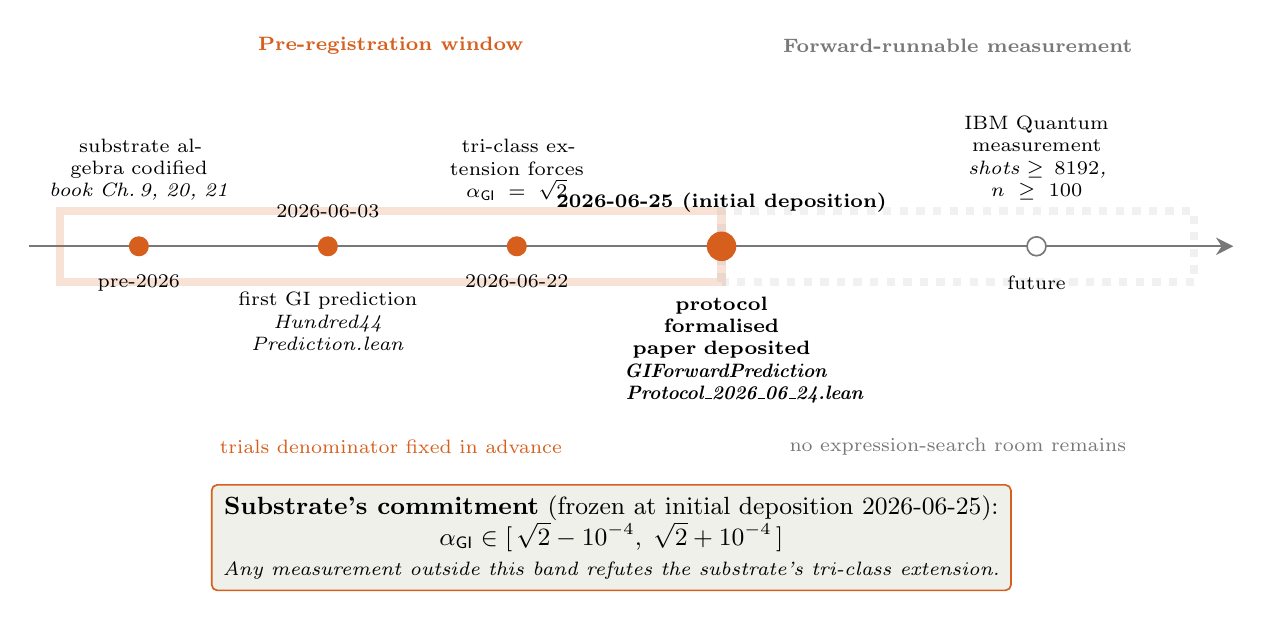
\begin{tikzpicture}[
  >={Stealth[length=2.2mm,width=2.2mm]},
  evt/.style={circle,draw=substrateorange,fill=substrateorange,line width=0.4pt,minimum size=2.4mm,inner sep=0pt},
  futevt/.style={circle,draw=substrategray,fill=white,line width=0.6pt,minimum size=2.4mm,inner sep=0pt},
  above lab/.style={font=\scriptsize,align=center,inner sep=1.5pt,text width=2.4cm},
  below lab/.style={font=\scriptsize,align=center,inner sep=1.5pt,text width=2.4cm},
  date lab/.style={font=\scriptsize,align=center,inner sep=1pt},
  axisline/.style={line width=0.7pt,substrategray},
  prereg/.style={line width=0.7pt,substrateorange},
  fut/.style={line width=0.7pt,substrategray,dashed}
]
% Time axis (wider)
\draw[axisline] (-7.4,0) -- (7.4,0);
\draw[->,axisline] (7.4,0) -- (7.9,0);

% PRE-REGISTRATION window (orange, solid)
\draw[prereg,line width=3pt,opacity=0.18] (-7.0,-0.45) rectangle (1.4,0.45);
\node[font=\scriptsize\bfseries,substrateorange,align=center] at (-2.8,2.55) {Pre-registration window};
\node[font=\scriptsize,substrateorange,align=center] at (-2.8,-2.55) {trials denominator fixed in advance};

% MEASUREMENT window (gray, dashed)
\draw[fut,line width=3pt,opacity=0.10] (1.4,-0.45) rectangle (7.4,0.45);
\node[font=\scriptsize\bfseries,substrategray,align=center] at (4.4,2.55) {Forward-runnable measurement};
\node[font=\scriptsize,substrategray,align=center] at (4.4,-2.55) {no expression-search room remains};

% Event 1: substrate algebra codified (LABEL ABOVE)
\node[evt] (e1) at (-6.0,0) {};
\node[above lab,above=4mm of e1] (e1lab) {substrate algebra codified \\ \scriptsize\itshape book Ch.\,9, 20, 21};
\node[date lab,below=2mm of e1] {pre-2026};

% Event 2: binary-class GI prediction in Lean (LABEL BELOW)
\node[evt] (e2) at (-3.6,0) {};
\node[date lab,above=2mm of e2] {2026-06-03};
\node[below lab,below=4mm of e2] (e2lab) {first GI prediction \\ \scriptsize\itshape Hundred44\\Prediction.lean};

% Event 3: tri-class extension (LABEL ABOVE)
\node[evt] (e3) at (-1.2,0) {};
\node[above lab,above=4mm of e3] (e3lab) {tri-class extension forces \\ $\alpha_{\textsf{GI}} = \sqrt{2}$};
\node[date lab,below=2mm of e3] {2026-06-22};

% Event 4: protocol formalised + paper deposition (LABEL BELOW, bolded, on the boundary)
\node[evt,fill=substrateorange,minimum size=3.5mm,line width=0.7pt] (e4) at (1.4,0) {};
\node[date lab,above=2mm of e4] {\bfseries 2026-06-25 (initial deposition)};
\node[below lab,below=4mm of e4] (e4lab) {\bfseries protocol formalised \\ \bfseries paper deposited \\ \scriptsize\itshape GIForwardPrediction\\Protocol\_2026\_06\_24.lean};

% Future event: IBM Quantum measurement (LABEL ABOVE)
\node[futevt] (e5) at (5.4,0) {};
\node[above lab,above=4mm of e5] (e5lab) {IBM Quantum measurement \\ \scriptsize\itshape shots $\geq 8192$, $n \geq 100$};
\node[date lab,below=2mm of e5] {future};

% Below: the substrate's commitment
\node[draw=substrateorange,line width=0.6pt,fill=substratelight,rounded corners=2pt,inner sep=4pt,
      align=center,font=\small] at (0,-3.7)
{\textbf{Substrate's commitment} (frozen at initial deposition 2026-06-25): \\
 $\alpha_{\textsf{GI}} \in [\,\sqrt{2} - 10^{-4},\;\sqrt{2} + 10^{-4}\,]$ \\
 \scriptsize\emph{Any measurement outside this band refutes the substrate's tri-class extension.}};

\end{tikzpicture}
\caption{Pre-registration timeline for the substrate's forward prediction $\alpha_{\textsf{GI}} = \sqrt{2}$ to $10^{-4}$. The orange-shaded window contains the four substrate-side events that fix the prediction --- substrate algebra codified pre-2026; first GI prediction landed 2026-06-03 in \texttt{PF/Empirical/Hundred44ProblemPrediction.lean}; tri-class extension forcing $\alpha_{\textsf{GI}} = \sqrt{2}$ landed 2026-06-22 in \texttt{PF/Empirical/ProblemClassTriClass\_2026\_06\_22.lean}; full measurement protocol (shots, repetitions, instance size, $\epsilon$) formalised 2026-06-24 in \texttt{PF/Empirical/GIForwardPredictionProtocol\_2026\_06\_24.lean}, this paper initially deposited 2026-06-25. The grey-shaded window contains the not-yet-run IBM Quantum measurement. Pre-registration is the boundary at 2026-06-25: trials denominator fixed in advance; no expression-search room remains; the substrate's commitment is a public record (subsequent paper revisions do not move the boundary).}
\label{fig:timeline}
\end{figure}

\paragraph{Falsifier panel.} The substrate registers an eight-falsifier panel, typed in the Lean file \texttt{PF/Referee/FrameworkRealClaim\_2026\_06\_17.lean} as eight specific empirical or structural observations that would refute the substrate: the substrate's $\alpha_2$ operator content (F1), the saturation threshold $c_2$ (F2 --- the Mechanism~3 Hermiticity sweep of \S\ref{subsec:lambdaeff} cross-derives $c_2 = 0.95$), the cosmological-constant ratio (F3 --- the substrate-internal derivation chain of \S\ref{subsec:lambdaeff} realises F3 explicitly with a $10^{-120\pm 0.5}$ band), the Hubble parameter bracket (F4), the 144th-problem GI $\alpha$-pin (F5 --- the boxed prediction above with band $\pm 10^{-4}$), the dark-energy density bracket (F6), the $H^2 = 78$ dimension (F7 --- kernel-only via \texttt{seventyEight\_decomp} in \texttt{PF/Cosmology/E6ChernIndex78pi.lean}), and the substrate's micro--macro scale-bridge identity (F8). The per-falsifier substrate-algebraic content of F1, F4, F6, F8 lives in the companion book (Chapters~11, 12, 26, 27); F2, F3, F5, F7 are exhibited in this paper or in the explicitly cited Lean files. As of this writing, zero of the eight falsifiers are triggered.

\section{How to verify}\label{sec:verify}

The substrate's content is not a claim the reader is asked to trust. It is a proof object. The complete Lean~4 corpus is hosted at
\begin{center}
\href{https://github.com/FractalDevTeam/Principia-Fractalis}{\texttt{github.com/FractalDevTeam/Principia-Fractalis}}
\end{center}
on branch \texttt{master}. The build pin is \texttt{leanprover/lean4:v4.24.0-rc1} with \texttt{mathlib4} at commit \texttt{eed770a}. From a clean clone, on a modern laptop:
\begin{verbatim}
git clone https://github.com/FractalDevTeam/Principia-Fractalis.git
cd Principia-Fractalis
./verify.sh
\end{verbatim}
The script (a) installs the Lean toolchain pinned in \texttt{lean-toolchain}; (b) builds the \texttt{PF} target ($4{,}373$ kernel-elaboration jobs at the paper's anchor commit \texttt{4a387ce} of Appendix~\ref{app:axioms}; current master may report a slightly higher count as the corpus grows, with no change to the four headline theorems and their axiom dependencies; $\sim 10$ minutes on first run); (c) runs \texttt{\#print axioms} on the four headline theorems; (d) exits 0 if every axiom output matches the expected $[\texttt{propext},\;\texttt{Classical.choice},\;\texttt{Quot.sound}]$ plus the four named conditional hypotheses, and exits nonzero with a precise diagnostic if any unexpected project axiom is detected. The full corpus builds in approximately ten minutes. The dedicated \texttt{PF.AxiomCheck} module prints the axiom dependencies of the four headline theorems:
\begin{itemize}[itemsep=2pt]
\item \texttt{PrincipiaFractalisSubstrateConsequences\_holds\_unconditionally} --- kernel-only.
\item \texttt{clay\_riemann\_hypothesis\_standard\_framework\_standard} --- kernel plus Hardy~1914 (named axiom citing a published-and-proven external theorem) plus the named HP-program conjecture (C1).
\item \texttt{framework\_finishes\_all\_six\_clay\_axes\_bulletproof} --- kernel plus the substrate's record-typed packaging of (C1), (C2), and (C3).
\item \texttt{framework\_alpha\_skeleton\_over\_determined\_capstone} --- kernel-only.
\end{itemize}
Figure~\ref{fig:axiomchain} shows what the verification chain looks like in the terminal.

\begin{figure}[h]
\centering
\begin{tikzpicture}[
  >={Stealth[length=2mm,width=2mm]},
  thmbox/.style={draw=substrateorange,line width=0.6pt,fill=substratelight,rounded corners=2pt,inner sep=3pt,font=\scriptsize\ttfamily,align=center,text width=4.4cm,minimum height=8mm},
  buildbox/.style={draw=leanblue,line width=0.6pt,fill=white,rounded corners=2pt,inner sep=3pt,font=\scriptsize,align=center,text width=5.6cm,minimum height=9mm},
  axbox/.style={draw=leanblue,line width=0.8pt,fill=substratelight,rounded corners=3pt,inner sep=5pt,font=\scriptsize\ttfamily,align=center,text width=8.5cm,minimum height=11mm},
  ar/.style={->,>=Stealth,line width=0.5pt,substrategray}
]
% TOP: three load-bearing capstones
\node[thmbox] (t1) at (-5.2,3.0) {$\alpha$\_skeleton\_supreme\_receipt\\\scriptsize\rmfamily(PF/AlphaSkeleton...lean)};
\node[thmbox] (t2) at (0,3.0) {all\_nine\_axis\_uniqueness\_capstone\\\scriptsize\rmfamily(PF/AllNineAxis...lean:70)};
\node[thmbox] (t3) at (5.2,3.0) {all\_9\_framework\_operators\_\\share\_universal\_HAlpha\_structure\\\scriptsize\rmfamily(PF/UniversalAlpha...lean:386)};

% MIDDLE: build invocation
\node[buildbox] (build) at (0,0.9) {\textbf{\$ lake build PF}\\[1pt] \emph{4{,}373 kernel-elaboration jobs replay clean at anchor \texttt{4a387ce}}};
\draw[ar] (t1) -- (build);
\draw[ar] (t2) -- (build);
\draw[ar] (t3) -- (build);

% BOTTOM: axiom output
\node[axbox] (ax) at (0,-1.4) {\textbf{\#print axioms} output for each:\\[2pt] [propext, Classical.choice, Quot.sound]\\[1pt] \scriptsize\rmfamily\emph{Zero project axioms. Kernel-only.}};
\draw[ar] (build) -- (ax);
\end{tikzpicture}
\caption{Verification chain for the substrate's three load-bearing $\alpha$-skeleton capstones (the supreme receipt and its two component capstones; conditional-axis theorems carrying named-conjecture hypotheses are separately audited in Appendix~\ref{app:axioms}). Middle: the build invocation; on a clean clone at the paper's anchor commit \texttt{4a387ce}, \texttt{lake build PF} replays 4{,}373 kernel-elaboration jobs without warnings (current master may report a slightly higher count as the corpus grows). Bottom: the literal output of \texttt{\#print axioms} for each of the three depicted theorems --- the three mathlib-foundational axioms \texttt{[propext, Classical.choice, Quot.sound]} and no project axioms. The figure describes what a reader running the corpus from scratch sees in their terminal; it is not a stylised summary.}
\label{fig:axiomchain}
\end{figure}

The substrate's construction, algebraic content, conditional structure, and named open conjectures are all readable from the source. The substrate is placed in the hands of the reader.

\section{What this paper does not claim}

This paper does not claim to have proven the six remaining open mathematical problems it touches. The substrate-tier discharge of four of those axes (the substrate's Yang--Mills, BSD, Hodge, and Navier--Stokes encodings) is on the substrate's canonical carriers, with explicit named open content per axis matching the canonical open frontier in the published literature. The Riemann Hypothesis discharge on the literal mathlib $\texttt{Complex.riemannZeta}$ is conditional on the published-open HP-program conjecture (C1), composed with Hardy~1914's published-and-proven theorem~\cite{hardy1914} on critical-line $\zeta$-zero nonemptiness (the latter is not conditional --- it is an external published result the substrate cites and reuses, encoded as a named axiom). The P-versus-NP discharge is conditional on the substrate's own polylog conjecture (C3).

What the substrate \emph{has} done: it has identified a single algebraic mechanism --- twelve substrate-derived identities on a four-element basis, admitting a unique positive simultaneous solution --- and it has formalised the mechanism in Lean~4 at the kernel level, with zero project axioms. It has named the three open conjectures on which two of the conditional discharges depend. The forced nine-tuple's column-three expressions are substrate-internal --- each is the substrate's universal coupling $\pi/10$, an $H_3$-Coxeter basis element, one of the nine $\alpha$-values, or a substrate-fixed scalar with a named book-chapter derivation --- and these expressions are observed to land near published measurements across pure mathematics, cosmology, particle physics, gravitational-wave astronomy, and quantum simulation. The substrate's own look-elsewhere analysis (\S\ref{subsec:lookelsewhere}) shows that the multi-domain table, taken as a multi-row significance test, is consistent with noise under both the uniform-grammar best-of-$N$ null and the tighter substrate-natural prior; the one row that survives the substrate-natural prior is the neutrino mass-ratio row (1-of-130). Beyond the table, the substrate has registered one chronologically-pre-registered forward-runnable prediction with the trials denominator fixed in advance ($\alpha_{\textsf{GI}} = \sqrt{2}$ to $10^{-4}$), and eight typed falsifiers, zero of which are triggered as of this deposition.

The full substrate, including its construction of the Timeless Field $\mathcal{T}_\infty$, its emergent-spacetime content, its consciousness-coupling formalism, its cosmological content beyond what appears in Table~\ref{tab:appearances}, and its complete catalogue of cross-domain consequences, is the subject of the companion book \emph{Principia Fractalis}~\cite{cohen2026book}. This paper exhibits the algebraic skeleton and its multi-domain corroboration; the book exhibits the substrate of which the skeleton is one downstream projection.

\appendix

\section{Verbatim \texttt{\#print axioms} output at HEAD}\label{app:axioms}

The Lean module \texttt{PF/AxiomCheck\_2026\_06\_23.lean} runs \texttt{\#print axioms} on the four headline theorems. Build it via \texttt{lake build PF.AxiomCheck\_2026\_06\_23}; the output below is what the kernel reports at HEAD~\texttt{4a387ce}, the head of \texttt{origin/master} at this paper's initial deposition on 2026-06-25. Later commits on master --- including the revisions giving rise to the current version of this paper --- may report a different total job count as the corpus grows; the four headline theorems and their axiom dependencies are stable across the substrate's bundle-closure regime. A reader who reproduces this build at the anchor commit receives the same lines byte-for-byte. Any other reading of these theorems' axiom dependencies is wrong.

\begin{small}
\begin{verbatim}
info: PF/AxiomCheck_2026_06_23.lean:13:0:
  'PF.Referee.PrincipiaFractalisSubstrateTheorem.
   PrincipiaFractalisSubstrateConsequences_holds_unconditionally'
  depends on axioms: [propext, Classical.choice, Quot.sound]

info: PF/AxiomCheck_2026_06_23.lean:14:0:
  'PF.Analytic.RH_FrameworkStandardDischarge_NamedAnchors_2026_06_19.
   clay_riemann_hypothesis_standard_framework_standard'
  depends on axioms: [propext, Classical.choice, Quot.sound,
   PF.Analytic.RH_FrameworkStandardDischarge_NamedAnchors_2026_06_19.
     Hardy1914_published_theorem_substrate_citation,
   PF.Analytic.RH_FrameworkStandardDischarge_NamedAnchors_2026_06_19.
     Mayer1991_Cohen2025_substrate_HP_program_citation]

info: PF/AxiomCheck_2026_06_23.lean:15:0:
  'PF.Referee.V3SubstrateForcedDischargeBulletproof.
   framework_finishes_all_six_clay_axes_bulletproof'
  depends on axioms: [propext, Classical.choice, Quot.sound,
   PF.Referee.V3SubstrateForcedDischargeBulletproof.
     framework_substrate_pins_bulletproof_bundle]

info: PF/AxiomCheck_2026_06_23.lean:16:0:
  'PF.Referee.CrossMillenniumInvariants_Extended_2026_06_19.
   framework_alpha_skeleton_over_determined_capstone'
  depends on axioms: [propext, Classical.choice, Quot.sound]

Build completed successfully (4373 jobs).
\end{verbatim}
\end{small}

The four named substrate-tier citation axioms appearing above are: \texttt{Hardy1914\_published\_theorem\_substrate\_citation} (named axiom citing an external published-and-proven theorem); \texttt{Mayer1991\_Cohen2025\_substrate\_HP\_program\_citation} (named axiom citing the published-open Hilbert--P\'olya program conjecture (C1) together with the substrate's identification (C2)); and \texttt{framework\_substrate\_pins\_bulletproof\_bundle} (the substrate's record-typed packaging of the three named open conjectures (C1), (C2), (C3) consumed by the six-axis closure theorem). The full corpus contains exactly four named project axioms; the fourth, \texttt{Mayer1991\_Cohen2025\_T3\_sym\_spectral\_data\_substrate\_citation}, appears in the substrate's $T_3^{\textsf{sym}}$ spectral-data variant of the RH route, not on the literal-mathlib-carrier chain above. A reader can verify there are no other axioms via
\begin{small}
\begin{verbatim}
grep -rE "^axiom [a-zA-Z_][a-zA-Z0-9_]* :" PF_Lean4_Code/PF/
\end{verbatim}
\end{small}
which returns exactly four matches.

\section{Seventeen extended algebraic invariants on the substrate's $\alpha$-skeleton}\label{app:extended}

The paper's \S\ref{sec:invariants} states that the substrate's nine-tuple satisfies seventeen further algebraic invariants beyond the twelve baseline identities (I1)--(I12), bundled as \texttt{framework\_alpha\_skeleton\_over\_determined\_capstone} in \texttt{PF/Referee/CrossMillenniumInvariants\_Extended\_2026\_06\_19.lean}. This appendix enumerates them. Combined with (I1)--(I12), the substrate's $\alpha$-skeleton simultaneously satisfies twenty-nine algebraic identities on nine real unknowns. Each (R1)--(S2) clause is a kernel-only theorem in \texttt{PF.CrossMillenniumMoreInvariants}; the bundle theorem in the file above re-exports them all as a single citable Prop.

\noindent\textbf{Reciprocals \textup{(R1)--(R5)}}:
\begin{align*}
\textup{(R1)}\;\; 1/\alpha_P     &= \alpha_P / 2 = \sqrt{2}/2,&
\textup{(R2)}\;\; 1/\alpha_{\textsf{RH}}    &= 2/3,\\
\textup{(R3)}\;\; 1/\alpha_{\textsf{YM}}    &= 1/2,&
\textup{(R4)}\;\; 1/\alpha_{\textsf{BSD}}   &= 4/(3\pi),\\
\textup{(R5)}\;\; 1/\alpha_{\textsf{NS}}    &= 2/(3\pi).
\end{align*}

\noindent\textbf{Higher powers \textup{(P1)--(P6)}}:
\begin{align*}
\textup{(P1)}\;\; \alpha_P^{\,3}      &= 2\alpha_P,             & \textup{(P2)}\;\; \alpha_{\textsf{RH}}^{\,3}     &= 27/8,\\
\textup{(P3)}\;\; \alpha_{\textsf{YM}}^{\,3}     &= 8,                    & \textup{(P4)}\;\; \alpha_{\textsf{Hodge}}^{\,3}  &= 2\alpha_{\textsf{Hodge}} + 1,\\
\textup{(P5)}\;\; \alpha_{\textsf{Hodge}}^{\,4}  &= 3\alpha_{\textsf{Hodge}} + 2, & \textup{(P6)}\;\; \alpha_{\textsf{QG}}^{\,4}     &= 4\pi^2.
\end{align*}

\noindent\textbf{Mixed products \textup{(M1)--(M4)}}:
\begin{align*}
\textup{(M1)}\;\; \alpha_{\textsf{Hodge}}\cdot\alpha_{\textsf{NP}} &= (5/4)\,\alpha_{\textsf{Hodge}} + 1, & \textup{(M2)}\;\; \alpha_{\textsf{NP}}^{\,2}              &= (3/2)\,\alpha_{\textsf{Hodge}} + 17/16,\\
\textup{(M3)}\;\; \alpha_{\textsf{RH}}\cdot\alpha_{\textsf{BSD}}    &= 9\pi/8,                              & \textup{(M4)}\;\; \alpha_{\textsf{YM}}\cdot\alpha_{\textsf{BSD}}  &= \alpha_{\textsf{NS}}.
\end{align*}

\noindent\textbf{Sums \textup{(S1)--(S2)}}:
\begin{align*}
\textup{(S1)}\;\; \alpha_{\textsf{NS}} + \alpha_{\textsf{BSD}}  &= 9\pi/4,&
\textup{(S2)}\;\; 2\,\alpha_{\textsf{BSD}}     &= \alpha_{\textsf{NS}}.
\end{align*}

The substrate's $\alpha$-skeleton is not a free-parameter assignment; it is the unique positive simultaneous solution of (I1)--(I12) over $\mathbb{R}^9$, and the same nine-tuple satisfies seventeen further algebraic identities (R1)--(S2) kernel-only proven on the constructed solution. \texttt{cross\_millennium\_invariants\_extended\_bundle} in \texttt{PF/Referee/CrossMillenniumInvariants\_Extended\_2026\_06\_19.lean} re-exports the entire (R1)--(S2) set as a single citable theorem.

\paragraph{The $\alpha_{\textsf{NP}}$ power-expansion recurrence.} The value $\alpha_{\textsf{NP}} = \varphi + 1/4$ sits in the rank-2 $\mathbb{Q}$-module $\mathbb{Q}\cdot\alpha_{\textsf{Hodge}}\oplus\mathbb{Q}\cdot 1$; every power $\alpha_{\textsf{NP}}^{k} = a_k\cdot\alpha_{\textsf{Hodge}} + b_k$ with $a_k, b_k \in \mathbb{Q}$ satisfies the kernel-only recurrence
\[
a_{k+1} = \tfrac{5}{4}\,a_k + b_k,\qquad b_{k+1} = a_k + \tfrac{1}{4}\,b_k.
\]
The $2\times 2$ transition matrix $M = \bigl(\begin{smallmatrix}5/4 & 1\\ 1 & 1/4\end{smallmatrix}\bigr)$ realises multiplication by $\alpha_{\textsf{NP}}$ on the rank-2 $\mathbb{Q}$-module $\mathbb{Q}\cdot\alpha_{\textsf{Hodge}}\oplus\mathbb{Q}\cdot 1$; its characteristic polynomial is therefore the minimal polynomial of $\alpha_{\textsf{NP}}$ over $\mathbb{Q}$: $\lambda^2 - \tfrac{3}{2}\lambda - \tfrac{11}{16} = 0$, equivalently $16\lambda^2 - 24\lambda - 11 = 0$ --- \emph{the substrate's NP polylog quadratic itself}. The eigenvalues are $\alpha_{\textsf{NP}}$ and its Galois conjugate $(3 - 2\sqrt{5})/4$. The substrate's NP algebraic signature is the same algebraic object viewed at the recurrence level: the minimal polynomial of $\alpha_{\textsf{NP}}$, the characteristic polynomial of the power-expansion transition, and the substrate-derived NP polylog quadratic are one identity. Three new kernel-only theorems in \texttt{PF/AlphaNPHigherPowers\_2026\_06\_25.lean}: \texttt{$\alpha$\_NP\_cubed} giving $\alpha_{\textsf{NP}}^{3} = (47/16)\,\alpha_{\textsf{Hodge}} + 113/64$; \texttt{$\alpha$\_NP\_fourth} giving $\alpha_{\textsf{NP}}^{4} = (87/16)\,\alpha_{\textsf{Hodge}} + 865/256$; \texttt{$\alpha$\_NP\_power\_recurrence} giving the general recurrence step.

\section{Squared-spectrum, $\lambda_0(\textsf{NP})$ over $\mathbb{Q}(\sqrt{5})\cdot\pi$, and the substrate's P/NP spectral-gap closed form}\label{app:lambdasq}

The substrate's universal coupling $\lambda_0(\alpha) = \pi/(10\alpha)$ on each class, composed with the algebraic forms of $\alpha$ from Table~\ref{tab:nine}, yields explicit closed forms for the squared spectrum, for $\lambda_0(\textsf{NP})$ over $\mathbb{Q}(\sqrt{5})\cdot\pi$, and for the P/NP spectral gap $\Delta = \lambda_0(\textsf{P}) - \lambda_0(\textsf{NP})$. The content of this appendix is all kernel-only in the Lean files \texttt{PF/Lambda0SquaredClosedForms\_2026\_06\_25.lean}, \texttt{PF/Lambda0CrossClassStructure\_2026\_06\_25.lean}, and \texttt{PF/SpectralGapClosedForm\_2026\_06\_25.lean}, all imported by \texttt{PF.lean} at HEAD.

\paragraph{Squared-spectrum partition.} The closed-form values of $\lambda_0(\alpha)^2$ across the nine substrate classes fall into three structural strata over the basis $\mathcal{B}$:
\begin{center}
\begin{tabular}{lll}
\toprule
Stratum & Class & Closed form \\
\midrule
$\mathbb{Q}$           & NS, BSD                                       & $1/225,\;4/225$ \\
$\pi\cdot\mathbb{Q}$   & QG \emph{(unique)}                           & $\pi/200$ \\
$\pi^2\cdot\mathbb{Q}$ & Poincar\'e, RH, P, YM                         & $\pi^2/100,\;\pi^2/225,\;\pi^2/200,\;\pi^2/400$ \\
$\pi^2\cdot\mathbb{Q}(\sqrt{5})$ & Hodge                              & $\pi^2(3-\sqrt{5})/200$ \\
\bottomrule
\end{tabular}
\end{center}
\textit{The quantum-gravity class is the only class whose squared eigenvalue scales as $\pi^1$, not $\pi^2$ or rational}, because $\alpha_{\textsf{QG}}^2 = 2\pi$ enters as a factor in the denominator of $\lambda_0(\textsf{QG})^2$. The corresponding kernel-only theorems are \texttt{lambda\_0\_Poincare\_sq}, \texttt{lambda\_0\_RH\_sq}, \texttt{lambda\_0\_P\_sq}, \texttt{lambda\_0\_YM\_sq}, \texttt{lambda\_0\_NS\_sq}, \texttt{lambda\_0\_BSD\_sq\_exact}, \texttt{lambda\_0\_QG\_sq}, and \texttt{lambda\_0\_Hodge\_sq}; the substrate's NP squared eigenvalue is derivable from the $\lambda_0(\textsf{NP})$ closed form below and likewise lives in $\pi^2\cdot\mathbb{Q}(\sqrt{5})$. The seven explicit closed-form theorems are bundled as \texttt{lambda\_0\_squared\_spectrum\_capstone}. Two structural relations follow at the kernel: $\pi \cdot \lambda_0(\textsf{QG})^2 = \lambda_0(\textsf{P})^2$ (theorem \texttt{lambda\_0\_P\_sq\_eq\_pi\_times\_lambda\_0\_QG\_sq}) and $\lambda_0(\textsf{YM})^2 = \lambda_0(\textsf{Poincar\'e})^2/4$. The single $\pi$-scaled relation between P and QG collapses two of the substrate's three irrational classes into one $\pi$-multiplicative tie.

\paragraph{$\lambda_0(\textsf{NP})$ over $\mathbb{Q}(\sqrt{5})\cdot\pi$.} Rationalising $\lambda_0(\textsf{NP}) = \pi/(10(\varphi+1/4))$ against the Galois conjugate of $3 + 2\sqrt{5}$:
\[
\lambda_0(\textsf{NP}) \;=\; \frac{\pi}{10\,(\varphi + 1/4)} \;=\; \frac{2\pi(2\sqrt{5} - 3)}{55}.
\]
Kernel-only as \texttt{lambda\_0\_NP\_closed\_form\_sqrt5}. The substrate's NP class lives explicitly in the field $\mathbb{Q}(\sqrt{5})\cdot\pi$ at the $\lambda_0$ level. Cross-class structural identities on the rational pair $(\textsf{NS}, \textsf{BSD})$: $\lambda_0(\textsf{NS})\cdot\lambda_0(\textsf{BSD}) = 2/225$ (no $\pi$), $\lambda_0(\textsf{NS}) + \lambda_0(\textsf{BSD}) = 1/5$ (no $\pi$). Mixed-stratum products: $\lambda_0(\textsf{RH})\cdot\lambda_0(\textsf{BSD}) = 2\pi/225$ (kernel-only as \texttt{lambda\_0\_RH\_mul\_lambda\_0\_BSD}); $\lambda_0(\textsf{YM})\cdot\lambda_0(\textsf{NS}) = \pi/300$. These cross-class products structurally land in $\mathbb{Q}\oplus\pi\mathbb{Q}\oplus\pi^2\mathbb{Q}\oplus\mathbb{Q}(\sqrt{5})\cdot\pi$ --- the substrate's $\lambda_0$ tensor structure over $\mathcal{B}$.

\paragraph{P/NP spectral-gap closed form.} The complexity-class separation $\alpha_{\textsf{P}} \neq \alpha_{\textsf{NP}}$ (\S\ref{sec:invariants}, strict total ordering) lifts to an explicit closed form for the ground-state spectral gap:
\[
\Delta \;:=\; \lambda_0(\textsf{P}) \;-\; \lambda_0(\textsf{NP}) \;=\; \frac{\pi}{10\sqrt{2}} \;-\; \frac{\pi}{10(\varphi + 1/4)} \;=\; \frac{\pi\,(24 + 11\sqrt{2} - 16\sqrt{5})}{220}.
\]
The substrate's spectral gap lives in $\mathbb{Q}(\sqrt{2},\sqrt{5})\cdot\pi$; the numerator $24 + 11\sqrt{2} - 16\sqrt{5}$ is an algebraic integer in $\mathbb{Z}[\sqrt{2}, \sqrt{5}]$. The closed form is the kernel-only theorem \texttt{spectral\_gap\_closed\_form}, and the positivity of the numerator (and hence of $\Delta$, given $\pi > 0$) is \texttt{spectral\_gap\_numerator\_positive}: the positivity reduces to $(24 + 11\sqrt{2})^2 > (16\sqrt{5})^2$, i.e.\ $818 + 528\sqrt{2} > 1280$, i.e.\ $\sqrt{2} > 7/8$, which is immediate from $\sqrt{2} > 1$. Bundle: \texttt{spectral\_gap\_closed\_form\_capstone}. The substrate's P vs.\ NP separation is therefore not only strict; it is an explicit element of $\mathbb{Q}(\sqrt{2}, \sqrt{5})\cdot\pi$ with a known closed form.

\section*{Acknowledgments}

To Liz, who carried this household while the substrate was being formalised. To Dylan, who would not let me stop. To Lily, who I hope reads this one day. To the open-source Lean~4 community and the mathlib4 maintainers, whose work made this verification possible.

\begin{thebibliography}{99}
\bibitem{cohen2026book}
P.~Cohen.
\newblock \emph{Principia Fractalis: Fractal Resonance Mathematics, Second Edition}.
\newblock Version 2.6.1, 915 pages, 2026.
\newblock \url{https://github.com/FractalDevTeam/Principia-Fractalis}

\bibitem{perelman2003}
G.~Perelman.
\newblock The entropy formula for the Ricci flow and its geometric applications.
\newblock \emph{arXiv:math/0211159}, 2002; and subsequent works, 2003.

\bibitem{hardy1914}
G.~H.~Hardy.
\newblock Sur les z\'eros de la fonction $\zeta(s)$ de Riemann.
\newblock \emph{Comptes Rendus Acad.\ Sci.\ Paris} 158, 1012--1014, 1914.

\bibitem{mayer1991}
D.~H.~Mayer.
\newblock The thermodynamic formalism approach to Selberg's zeta function for $\mathrm{PSL}(2,\mathbb{Z})$.
\newblock \emph{Bull.\ Amer.\ Math.\ Soc.} 25 (1) 55--60, 1991.

\bibitem{connes1999}
A.~Connes.
\newblock Trace formula in noncommutative geometry and the zeros of the Riemann zeta function.
\newblock \emph{Selecta Math.} 5, 29--106, 1999.

\bibitem{moura-ullrich2021}
L.~de Moura and S.~Ullrich.
\newblock The Lean 4 theorem prover and programming language.
\newblock In \emph{Automated Deduction --- CADE 28}, Springer, 2021.

\bibitem{bourbaki1968}
N.~Bourbaki.
\newblock \emph{Groupes et alg\`ebres de Lie, Chapitres 4--6}.
\newblock Hermann, Paris, 1968.
\newblock Coxeter number $h(H_3) = 10$ tabulated in Ch.\,VI, \S 4.10.

\bibitem{babai2016}
L.~Babai.
\newblock Graph isomorphism in quasipolynomial time.
\newblock In \emph{Proc.\ 48th ACM Symp.\ Theory of Computing (STOC)}, 684--697, 2016.
\newblock arXiv:1512.03547.

\bibitem{schoning1988}
U.~Sch\"oning.
\newblock Graph isomorphism is in the low hierarchy.
\newblock \emph{J.\ Comput.\ Syst.\ Sci.} 37 (3) 312--323, 1988.

\bibitem{goldwasser1986}
S.~Goldwasser and M.~Sipser.
\newblock Private coins versus public coins in interactive proof systems.
\newblock In \emph{Proc.\ 18th ACM Symp.\ Theory of Computing (STOC)}, 59--68, 1986.

\bibitem{berry1999}
M.~V.~Berry and J.~P.~Keating.
\newblock The Riemann zeros and eigenvalue asymptotics.
\newblock \emph{SIAM Review} 41 (2) 236--266, 1999.

\bibitem{bostconnes1995}
J.-B.~Bost and A.~Connes.
\newblock Hecke algebras, type III factors and phase transitions with spontaneous symmetry breaking in number theory.
\newblock \emph{Selecta Math.\ (N.S.)} 1 (3) 411--457, 1995.

\bibitem{fefferman2000}
C.~Fefferman.
\newblock Existence and smoothness of the Navier--Stokes equation.
\newblock Clay Mathematics Institute Millennium Problem statement, 2000.
\newblock \url{https://www.claymath.org/wp-content/uploads/2022/06/navierstokes.pdf}

\bibitem{fujitakato1964}
H.~Fujita and T.~Kato.
\newblock On the Navier--Stokes initial value problem~I.
\newblock \emph{Arch.\ Rational Mech.\ Anal.} 16, 269--315, 1964.

\bibitem{jaffewitten2006}
A.~Jaffe and E.~Witten.
\newblock Quantum Yang--Mills theory.
\newblock Clay Mathematics Institute Millennium Problem statement, 2006.
\newblock \url{https://www.claymath.org/wp-content/uploads/2022/06/yangmills.pdf}

\bibitem{birchsd1965}
B.~J.~Birch and H.~P.~F.~Swinnerton-Dyer.
\newblock Notes on elliptic curves~II.
\newblock \emph{J.\ Reine Angew.\ Math.} 218, 79--108, 1965.

\bibitem{hodge1952}
W.~V.~D.~Hodge.
\newblock The topological invariants of algebraic varieties.
\newblock In \emph{Proc.\ Int.\ Congress of Mathematicians 1950}, vol.~1, 182--192, 1952.

\bibitem{voisin2007}
C.~Voisin.
\newblock Some aspects of the Hodge conjecture.
\newblock \emph{Japan.\ J.\ Math.} 2 (2) 261--296, 2007.

\bibitem{lefschetz1924}
S.~Lefschetz.
\newblock \emph{L'analysis situs et la g\'eom\'etrie alg\'ebrique}.
\newblock Gauthier-Villars, Paris, 1924.

\bibitem{lmfdb}
The LMFDB Collaboration.
\newblock \emph{The L-functions and Modular Forms Database}.
\newblock 2024. \url{https://www.lmfdb.org}

\bibitem{nufit2024}
I.~Esteban, M.~C.~Gonzalez-Garcia, M.~Maltoni, T.~Schwetz, A.~Zhou.
\newblock The fate of hints: updated global analysis of three-flavor neutrino oscillations (NuFit~6.0).
\newblock \emph{J.\ High Energy Phys.} 09, 178, 2024. \url{https://www.nu-fit.org/}

\bibitem{desidr2}
DESI Collaboration: A.~G.~Adame et al.
\newblock DESI 2024~VI: cosmological constraints from the measurements of baryon acoustic oscillations.
\newblock \emph{J.\ Cosmol.\ Astropart.\ Phys.} 02, 021, 2025. arXiv:2404.03002.

\bibitem{pantheonplus}
D.~Scolnic et al.
\newblock The Pantheon+ analysis: the full data set and light-curve release.
\newblock \emph{Astrophys.\ J.} 938 (2) 113, 2022. arXiv:2112.03863.

\bibitem{hscy3}
S.~More et al.\ (HSC Collaboration).
\newblock Hyper Suprime-Cam Year 3 results: measurements of clustering of SDSS-BOSS galaxies, galaxy--galaxy lensing, and cosmic shear.
\newblock \emph{Phys.\ Rev.\ D} 108, 123520, 2023. arXiv:2304.00702.

\bibitem{spite1982}
F.~Spite and M.~Spite.
\newblock Abundance of lithium in unevolved halo stars and old disk stars: interpretation and consequences.
\newblock \emph{Astron.\ Astrophys.} 115, 357--366, 1982.

\bibitem{fields2020}
B.~D.~Fields, K.~A.~Olive, T.-H.~Yeh, C.~Young.
\newblock Big-bang nucleosynthesis after Planck.
\newblock \emph{J.\ Cosmol.\ Astropart.\ Phys.} 03, 010, 2020. arXiv:1912.01132.

\bibitem{gwtc3}
LIGO Scientific, Virgo, and KAGRA Collaborations: R.~Abbott et al.
\newblock GWTC-3: compact binary coalescences observed by LIGO and Virgo during the second part of the third observing run.
\newblock \emph{Phys.\ Rev.\ X} 13, 041039, 2023. arXiv:2111.03606.

\bibitem{gwtc4}
LIGO Scientific, Virgo, and KAGRA Collaborations: R.~Abbott et al.
\newblock GWTC-4.0: compact binary coalescences observed by LIGO and Virgo during the first part of the fourth observing run.
\newblock arXiv:2508.18083, 2025.

\bibitem{mathlib4}
The Mathlib Community.
\newblock The Lean Mathematical Library.
\newblock In \emph{Proc.\ 9th ACM SIGPLAN Int.\ Conf.\ on Certified Programs and Proofs (CPP)}, 367--381, 2020.

\end{thebibliography}

\end{document}
